\documentclass[table,xcdraw,dvipsnames]{beamer}
% \documentclass[mathserif]{beamer}
\usepackage{tikz}
\usetikzlibrary{arrows.meta}
\definecolor{my-grey}{RGB}{220,220,220}
\definecolor{myDarkRed}{RGB}{153,0,0}
\definecolor{myLightRed}{RGB}{255,102,102}
\definecolor{myDarkBlue}{RGB}{0,0,255}
\definecolor{myLightBlue}{RGB}{102,178,255}
\usepackage{booktabs}

\usetheme{Frankfurt}
\usecolortheme{beaver}
\usepackage{abraces}
\usepackage{marvosym}
\usepackage{multirow}
\usepackage{textpos}
\usepackage{amsmath, amssymb, bm}
%\usepackage{kbordermatrix}
\usepackage{tikz}
\usetikzlibrary{positioning}
%% \usepackage{euler}
\usepackage{animate}
\newcommand{\gooditem}[1]{\setbeamercolor{item}{fg=Green}\item #1} 
\newcommand{\pooritem}[1]{\setbeamercolor{item}{fg=Red}\item #1} 
\usepackage[normalem]{ulem}
% \usepackage[table,xcdraw,dvipsnames]{xcolor}

\newcommand*\rot[1]{\rotatebox{90}{#1}}

%\everymath{\displaystyle}
%\everymath{\color{Blue}}


\makeatletter
\setbeamertemplate{footline}
{
  \leavevmode%
  \hbox{%
  \begin{beamercolorbox}[wd=.50\paperwidth,ht=2.25ex,dp=1ex,center]{author in head/foot}%
    \usebeamerfont{author in head/foot}\insertshortauthor%% \beamer@ifempty{\insertshortinstitute}{}{(\insertshortinstitute)}
  \end{beamercolorbox}%
  \hskip2pt%
  \begin{beamercolorbox}[wd=.50\paperwidth,ht=2.25ex,dp=1ex,center]{title in head/foot}%
    \usebeamerfont{title in head/foot}\insertshorttitle~~~~~~~~~~~~~~~~\insertframenumber
  \end{beamercolorbox}%
  %% \begin{beamercolorbox}[wd=.20\paperwidth,ht=2.25ex,dp=1ex,right]{date in head/foot}%
  %%   \usebeamerfont{date in head/foot}\insertshortdate{}\hspace*{2em}
  %%   \insertframenumber\hspace*{2ex} 
  %% \end{beamercolorbox}
}%
  \vskip0pt%
}
\makeatother



\def\checkmark{\tikz\fill[scale=0.4](0,.35) -- (.25,0) -- (1,.7) -- (.25,.15) -- cycle;} 

\definecolor{lightblue}{rgb}{0.145,0.6666,1} % Defines the color used for content box headers
\definecolor{Red}{rgb}{0.9,0.15,0}
\definecolor{Blue}{rgb}{0.1,0.3,1}
% \definecolor{Blue}{rgb}{0.1,0.7,1}
\definecolor{Green}{rgb}{0.3,0.8,0.15}
\definecolor{Lightgray}{rgb}{0.86,0.86,0.86}
\setbeamercolor{block title}{bg=Red!30,fg=black}


\title[Covid-19 Mortality Age-patterns$\qquad\qquad\qquad$]
{\LARGE{Exploratory analysis on \\COVID-19 Mortality Age-patterns}} 


\author[C.G.~Camarda$\qquad\quad\qquad\quad\qquad\quad\qquad\quad\qquad\quad$April 2021]
{\large{\sl{Carlo Giovanni Camarda}}\\
	\scriptsize{\color{Blue}\texttt{sites.google.com/site/carlogiovannicamarda}}\\
	
\includegraphics[scale=0.19]{ined_Hs_couleur.jpg}      \\
	\scriptsize{Institut National d'\'Etudes D\'emographiques,
		France}}


\date[Apr 2021]{
$\,$\\$\,$\\ \textsl{TAG Working Group I, Meeting IV}\\
$\,$\\
\vspace{0.1cm}
\footnotesize{April 30th, 2021}} % (optional) 

\beamertemplatenavigationsymbolsempty
\begin{document}

\begin{frame}[plain]
\titlepage
\end{frame}

\addtobeamertemplate{frametitle}{}{%
\begin{textblock*}{100mm}(0.999\textwidth,-1.4cm)

\includegraphics[scale=0.07]{ined_Hs_couleur}
\end{textblock*}}

% \section*{}
% \begin{frame}{Outline}
%   \tableofcontents
% \end{frame}

% % table of contents only at the beginning
% \section[Outline]{}
% \frame{
% \frametitle{Outline}
% \tableofcontents
% }

% table of contents popping up at
% the beginning of each subsection:
\AtBeginSection[] {
  \begin{frame}<beamer>{Outline}
    % \begin{small}
    \tableofcontents[currentsection]
    % \end{small}
  \end{frame}
}


\begin{frame}[fragile]\frametitle{Data and models}
	\vspace{-0.2cm}
\begin{itemize}
	\item Data:
	\begin{itemize}
		\item a subset of COVerAGE-DB with 100+ deaths
		\item either both sex or males and females separately
		\item scaled to JHU total on Dec 31, 2020
	\end{itemize}
\medskip
	\item Log-mortality over age $x$, for population $p$ and sex $s$:
	\medskip
	
	{\color{Red}\textsl{C-PCLM}}: Population-specific, sexes combined
	\begin{footnotesize}
	$$\eta(x,p) = \eta^{p}(x)$$
	\end{footnotesize}
%\medskip

	{\color{Blue}\textsl{S-PCLM}}: Population-sex-specific 
	\begin{footnotesize}
	$$\eta(x,p,s) = \eta^{p,s}(x)$$
	\end{footnotesize}
%\medskip

{\color{Green}\textsl{A-PCLM}}: An additive approach:
\begin{footnotesize}
$$
\eta(x,p,s) = \eta^{0}(x) + s(x) + \delta^{p}(x)
$$
\vspace{-0.5cm}
\begin{itemize}
	\item[$\eta^{0}(x)$]: reference mortality
	\item[$s(x)$]: sex factor
	\item[$\delta^{p}(x)$]: population-specific deviance
\end{itemize}
\end{footnotesize}
\end{itemize}
	
\end{frame}


\begin{frame}[fragile]\frametitle{Hierarchical $k$-means clustering on different outcomes}
	\vspace{-0.2cm}
		
		{\color{Red}\textsl{C-PCLM}}: Sexes combined rate-of-aging
				\begin{footnotesize}
		$$\frac{d\, \eta^{p}(x)} {d \,x}$$
		\vspace{-0.3cm}
		\begin{itemize}
	\gooditem[\textbf{+}] available for more populations \& more robust
	\pooritem[\textbf{--}] mixture of eventual different patterns
\end{itemize}
		\end{footnotesize}

		\bigskip
		
		{\color{Blue}\textsl{S-PCLM}}: Sex-specific rate-of-aging, then combined
			\begin{footnotesize}
		$$\left[\frac{d\, \eta^{p,s=F}(x)} {d\, x} ; \frac{d\, \eta^{p,s=M}(x)} {d\, x}\right]$$ 
		\vspace{-0.3cm}
		\begin{itemize}
			\gooditem[\textbf{+}] enforce both sexes to be included in the same group
			\pooritem[\textbf{--}] less populations with available data by sex
		\end{itemize}
			\end{footnotesize}
		\bigskip
		
		{\color{Green}\textsl{A-PCLM}}: population-specific deviance
				\begin{footnotesize}
		$$
		\delta^{p}(x)
		$$
		\vspace{-0.4cm}
		\begin{itemize}
			\gooditem[\textbf{+}] all data estimated within a single model \& control for sex
			\pooritem[\textbf{--}] slightly more complex interpretation 
		\end{itemize}
			\end{footnotesize}
\end{frame}


\begin{frame}[fragile]\frametitle{{\color{Red}\textsl{C-PCLM}}}
	%
	\only<1>{
		\vspace{-0.5cm}
		\begin{center}
			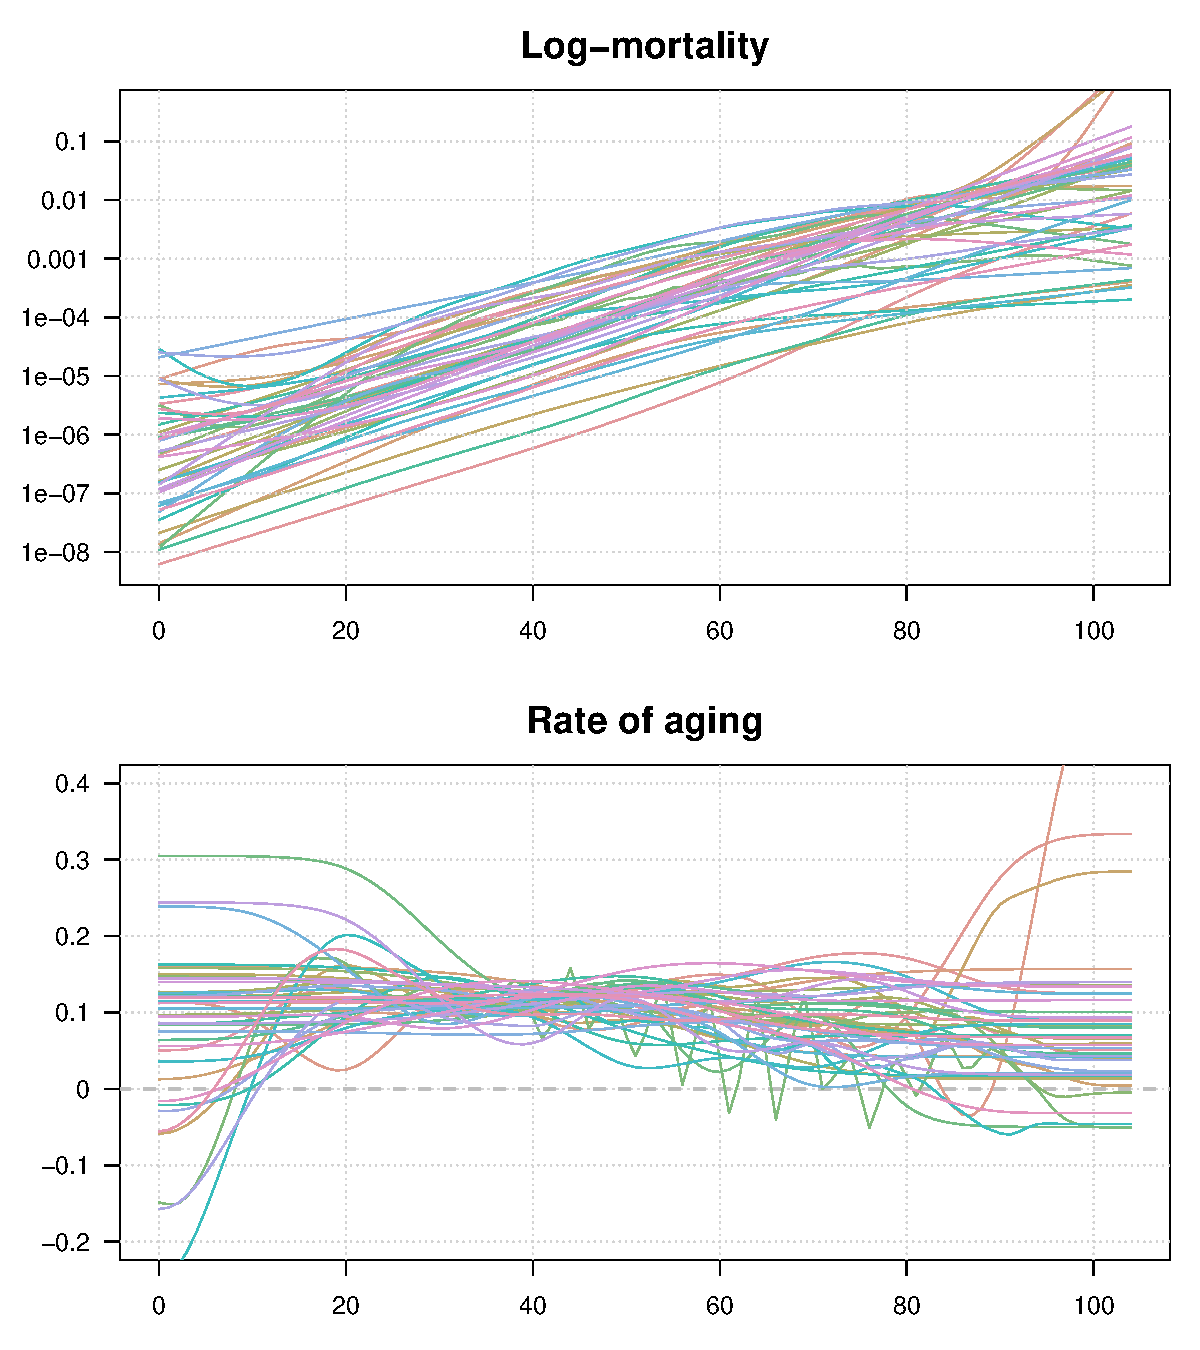
\includegraphics[scale=.35]{Figures/CombData.pdf}
		\end{center}
	}
	\only<2>{
		\begin{columns}
			\begin{column}{5cm}
				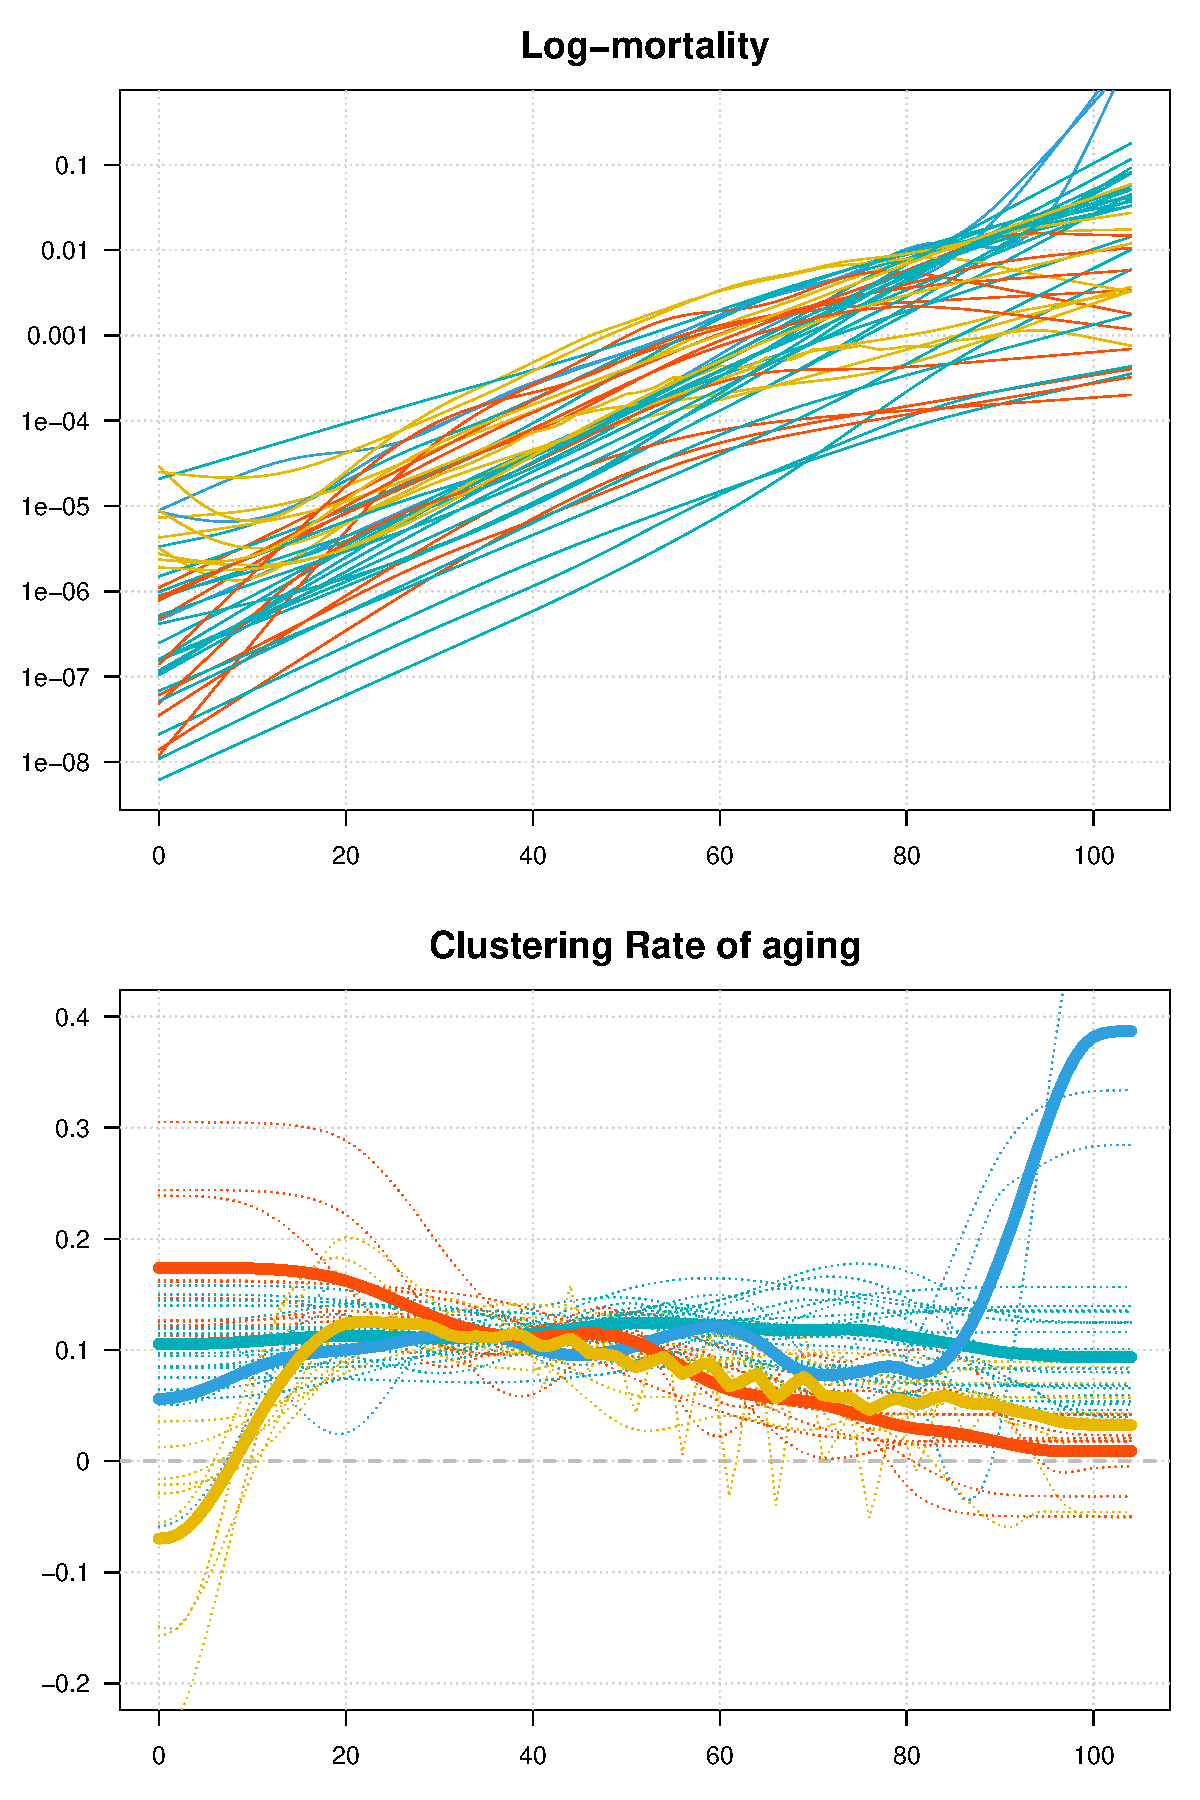
\includegraphics[scale=.23]{Figures/CombClust.pdf}
				\begin{tiny}
					Explained variance PC1+PC2: 40.1\% + 22.1\%
				\end{tiny}
			\end{column}
			\begin{column}{5cm}
				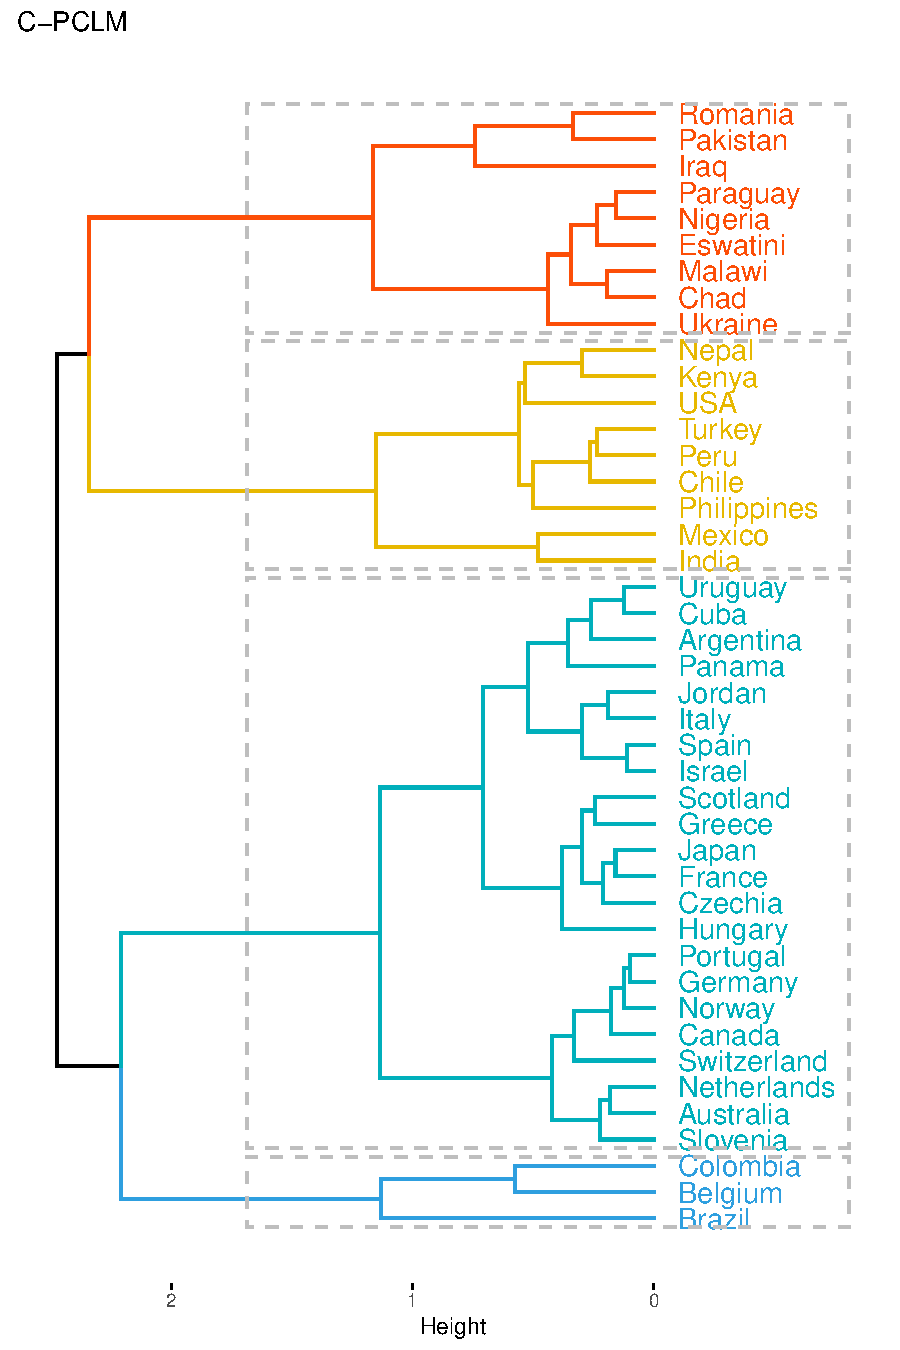
\includegraphics[scale=.35]{Figures/CombDendo.pdf}
			\end{column}
		\end{columns}
	}
\end{frame}


\begin{frame}[fragile]\frametitle{{\color{Blue}\textsl{S-PCLM}}\only<3>{ vs.~{\color{Red}\textsl{C-PCLM}}}}
	%\vspace{-0.5cm}
	\only<1>{
		\begin{center}
			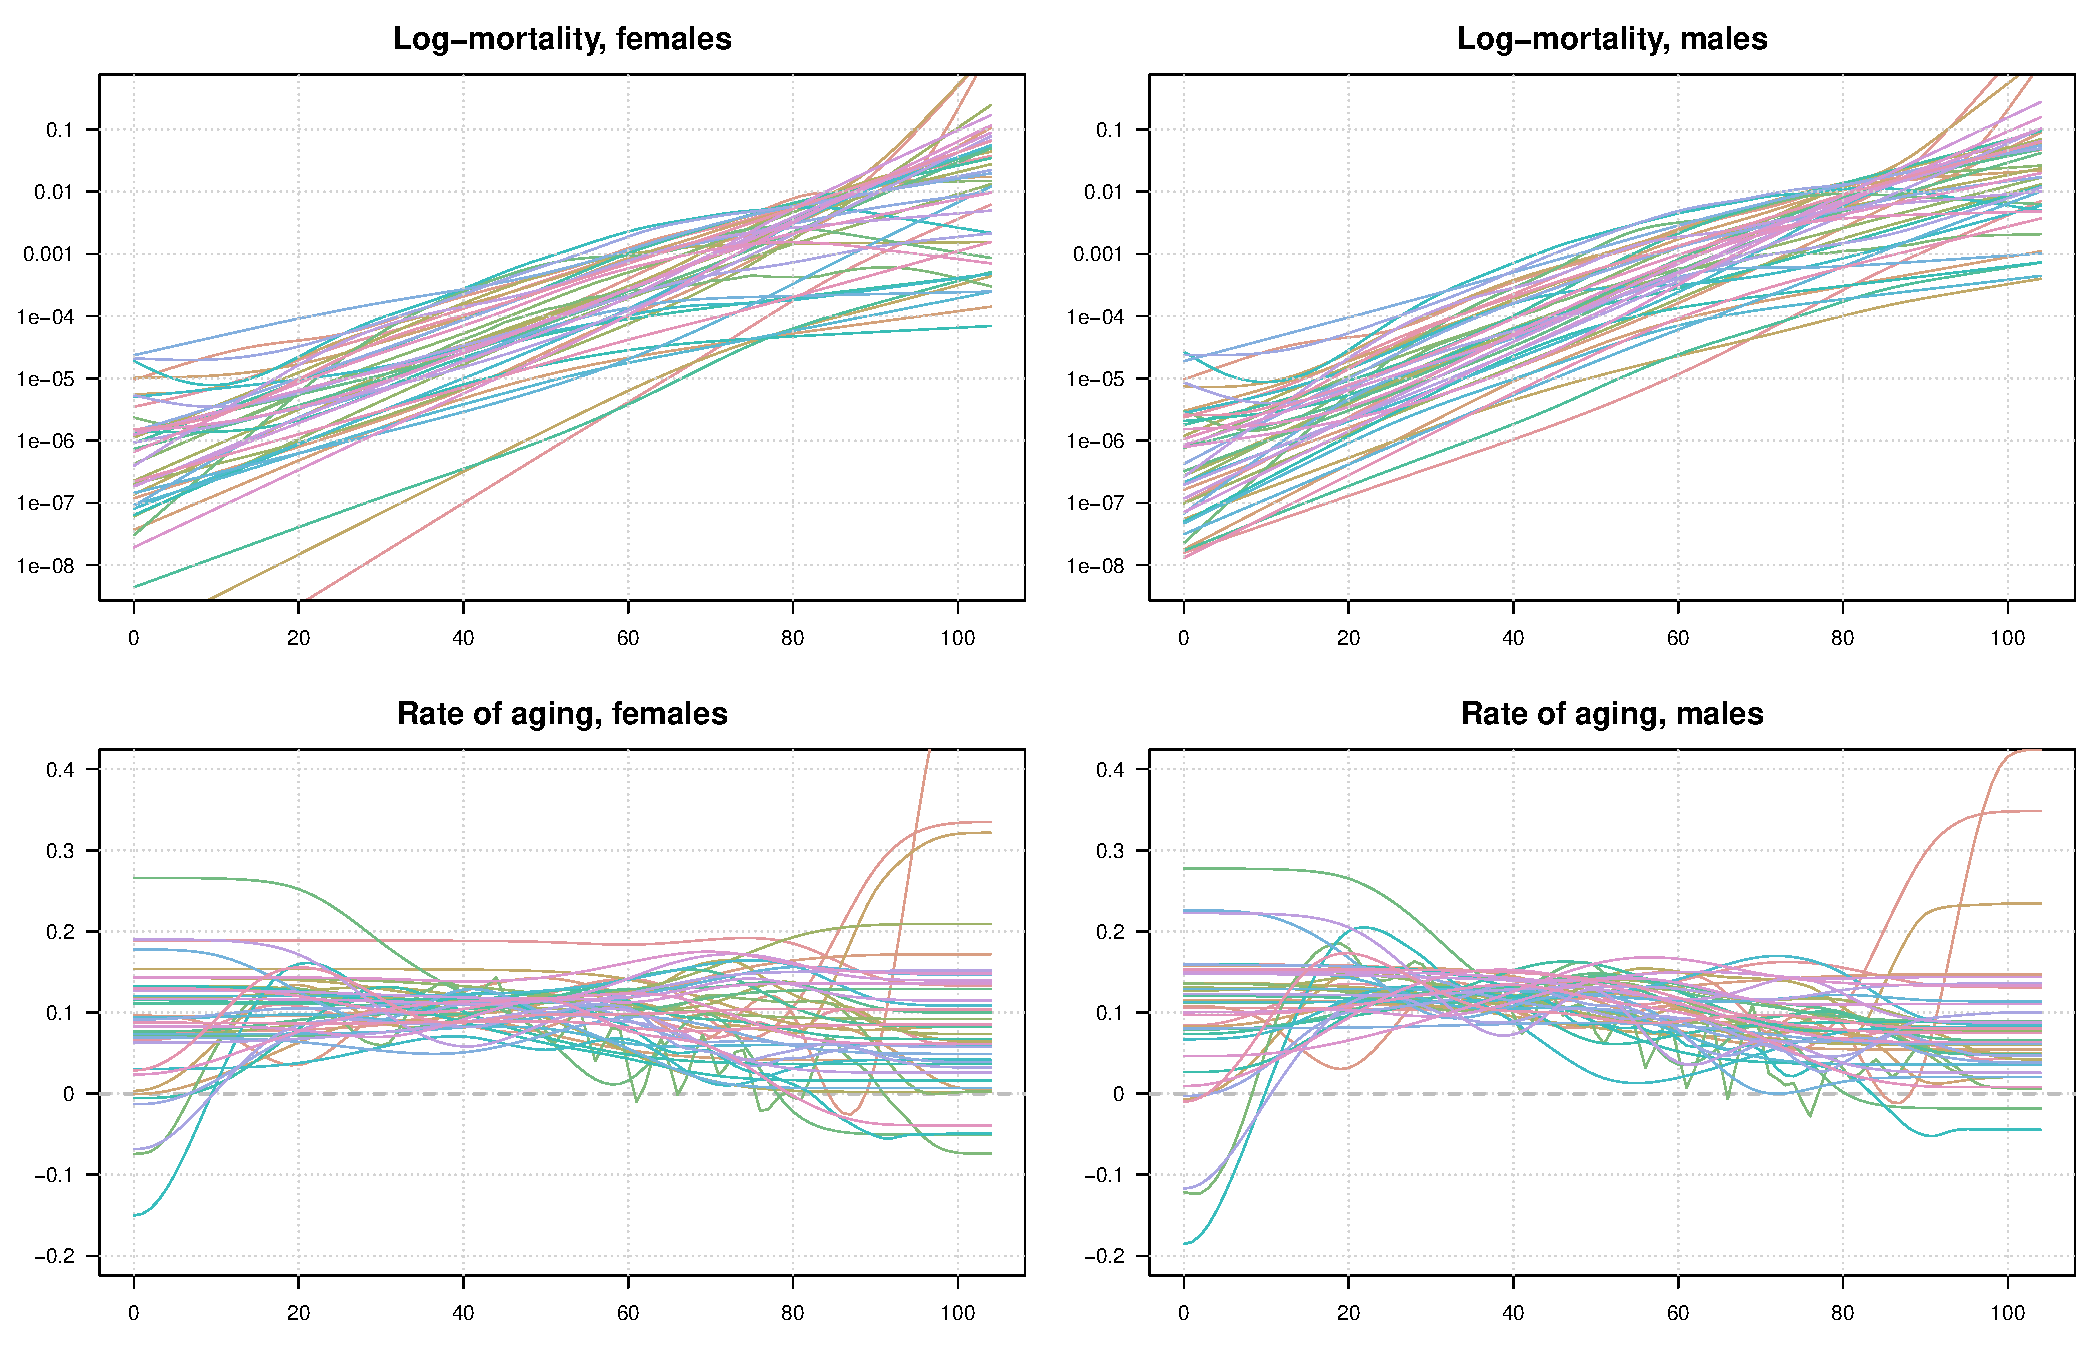
\includegraphics[scale=.3]{Figures/SexData.pdf}
		\end{center}
	}
	\only<2>{
	\begin{center}
		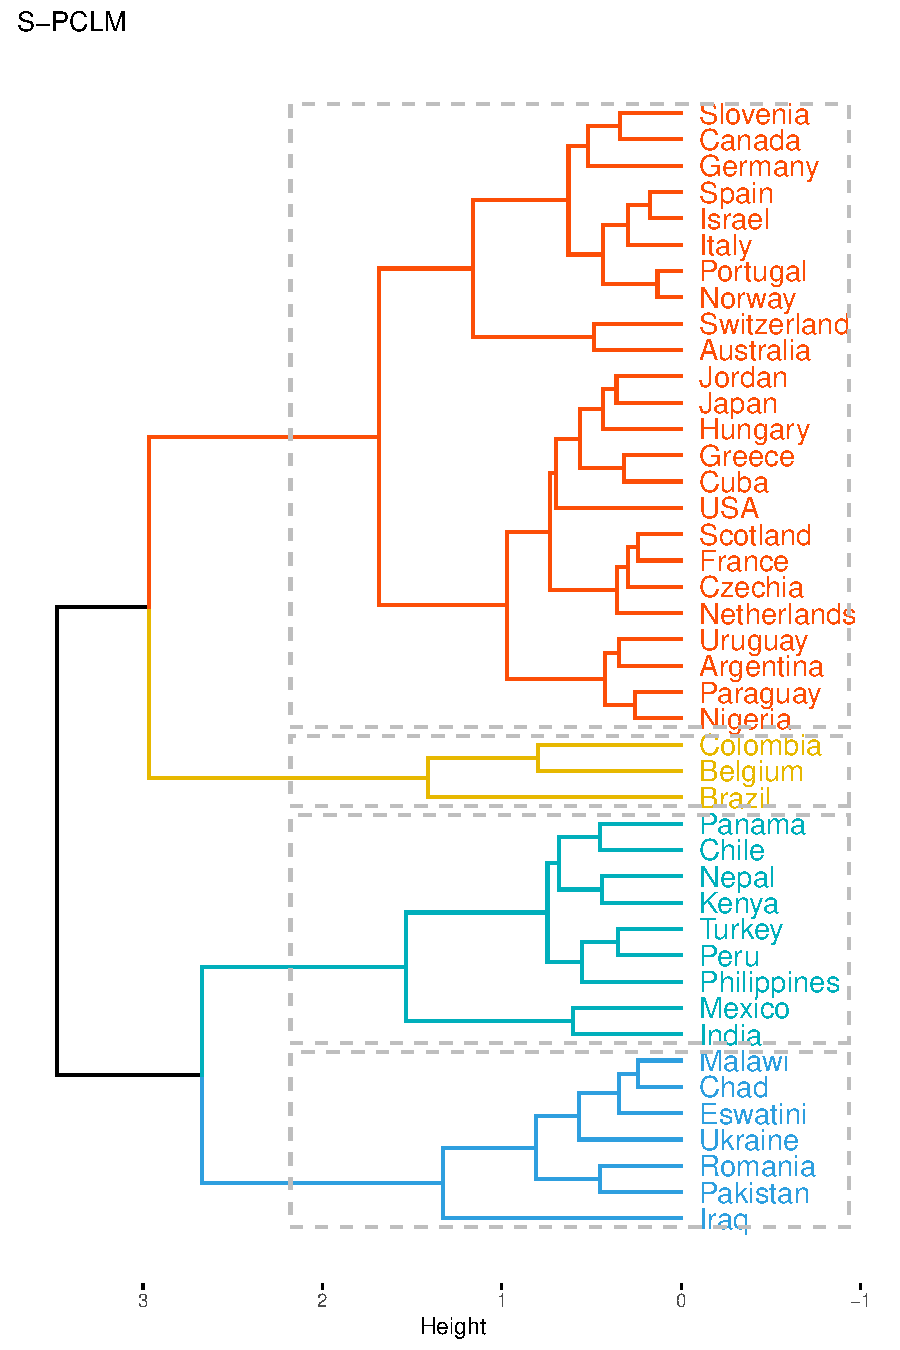
\includegraphics[scale=.3]{Figures/SexDendo.pdf}
	\end{center}
				\begin{tiny}
	Explained variance PC1+PC2: 37.6\% + 22.3\%
\end{tiny}
}
	\only<3>{
		\begin{columns}
			\begin{column}{5cm}
				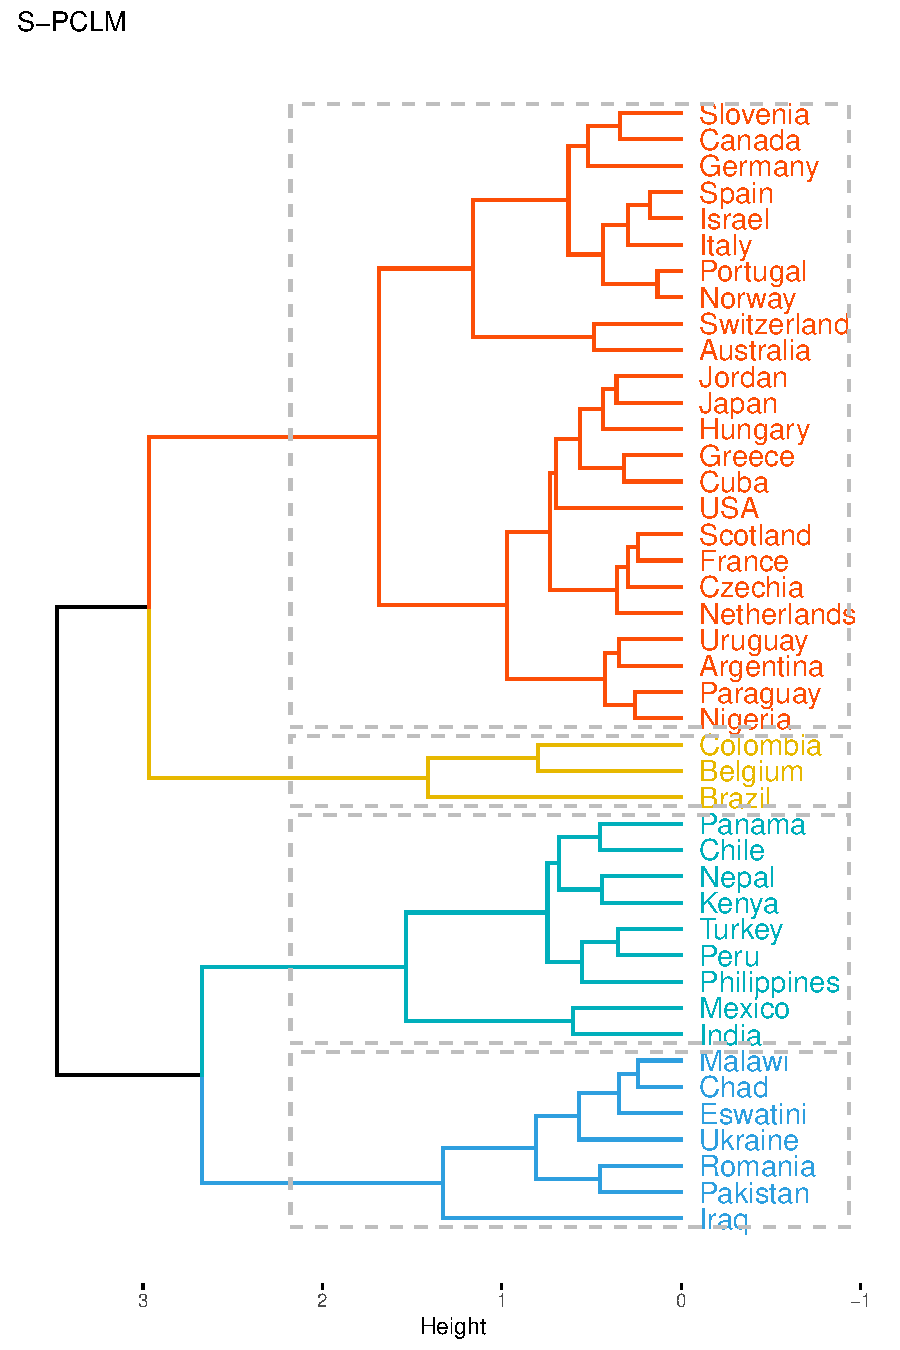
\includegraphics[scale=.3]{Figures/SexDendo.pdf}
			\end{column}
		
			\begin{column}{5cm}
				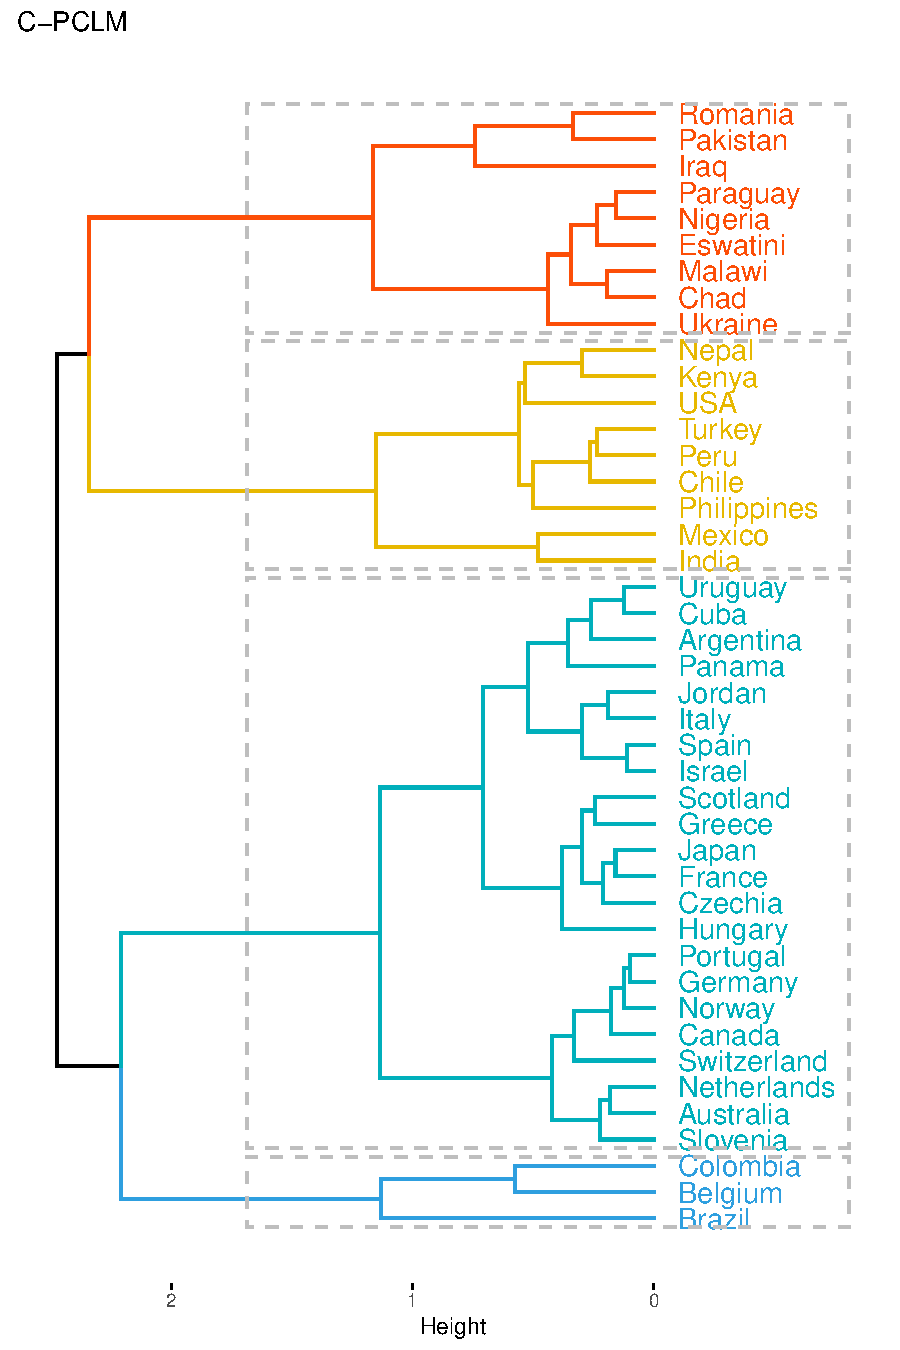
\includegraphics[scale=.3]{Figures/CombDendo.pdf}
			\end{column}
		\end{columns}
	}
\end{frame}


\begin{frame}[fragile]\frametitle{{\color{Green}\textsl{A-PCLM}}}
	%
	\only<1>{
		\vspace{-0.5cm}
		\begin{center}
			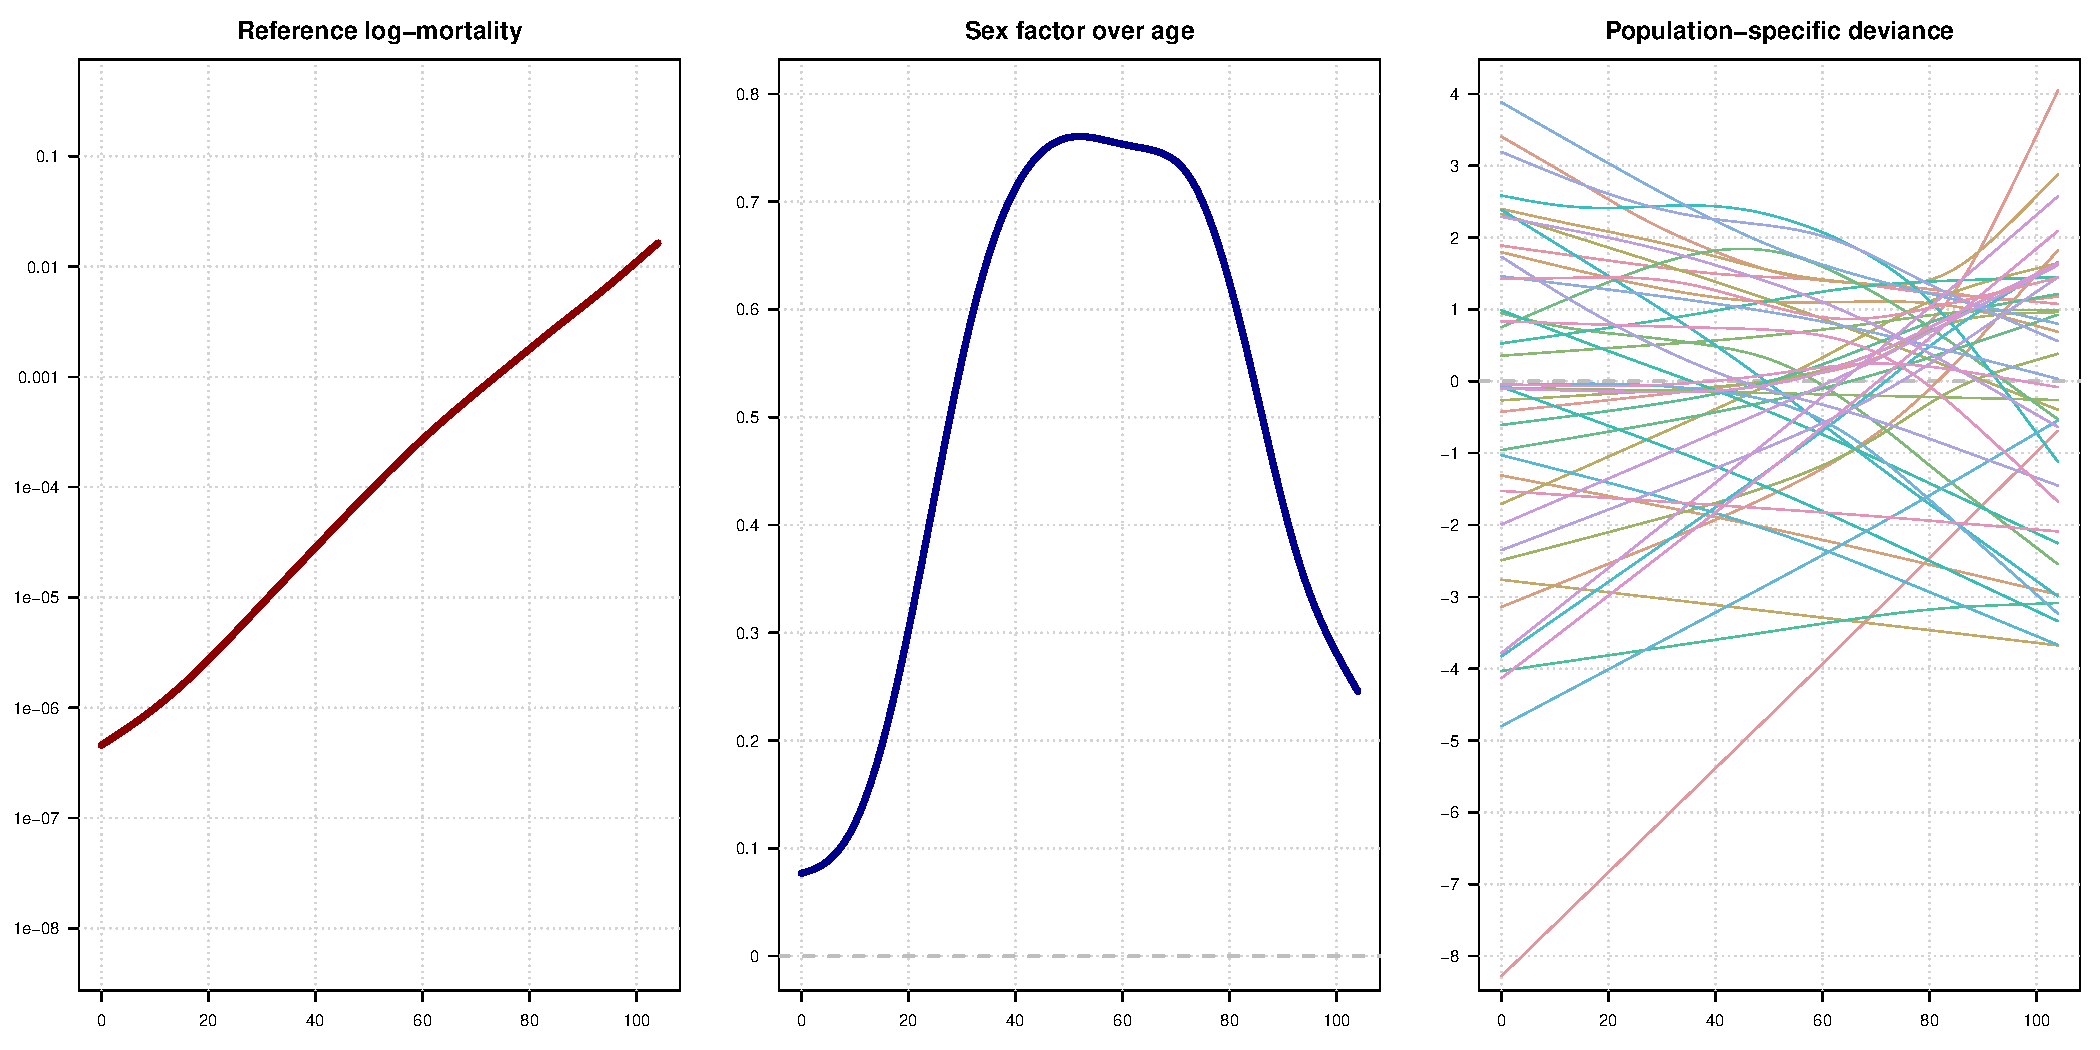
\includegraphics[scale=.3]{Figures/HierOut.pdf}% 77.3 + 21.5
		\end{center}
	}
	\only<2>{
	\begin{columns}
		\begin{column}{5cm}
			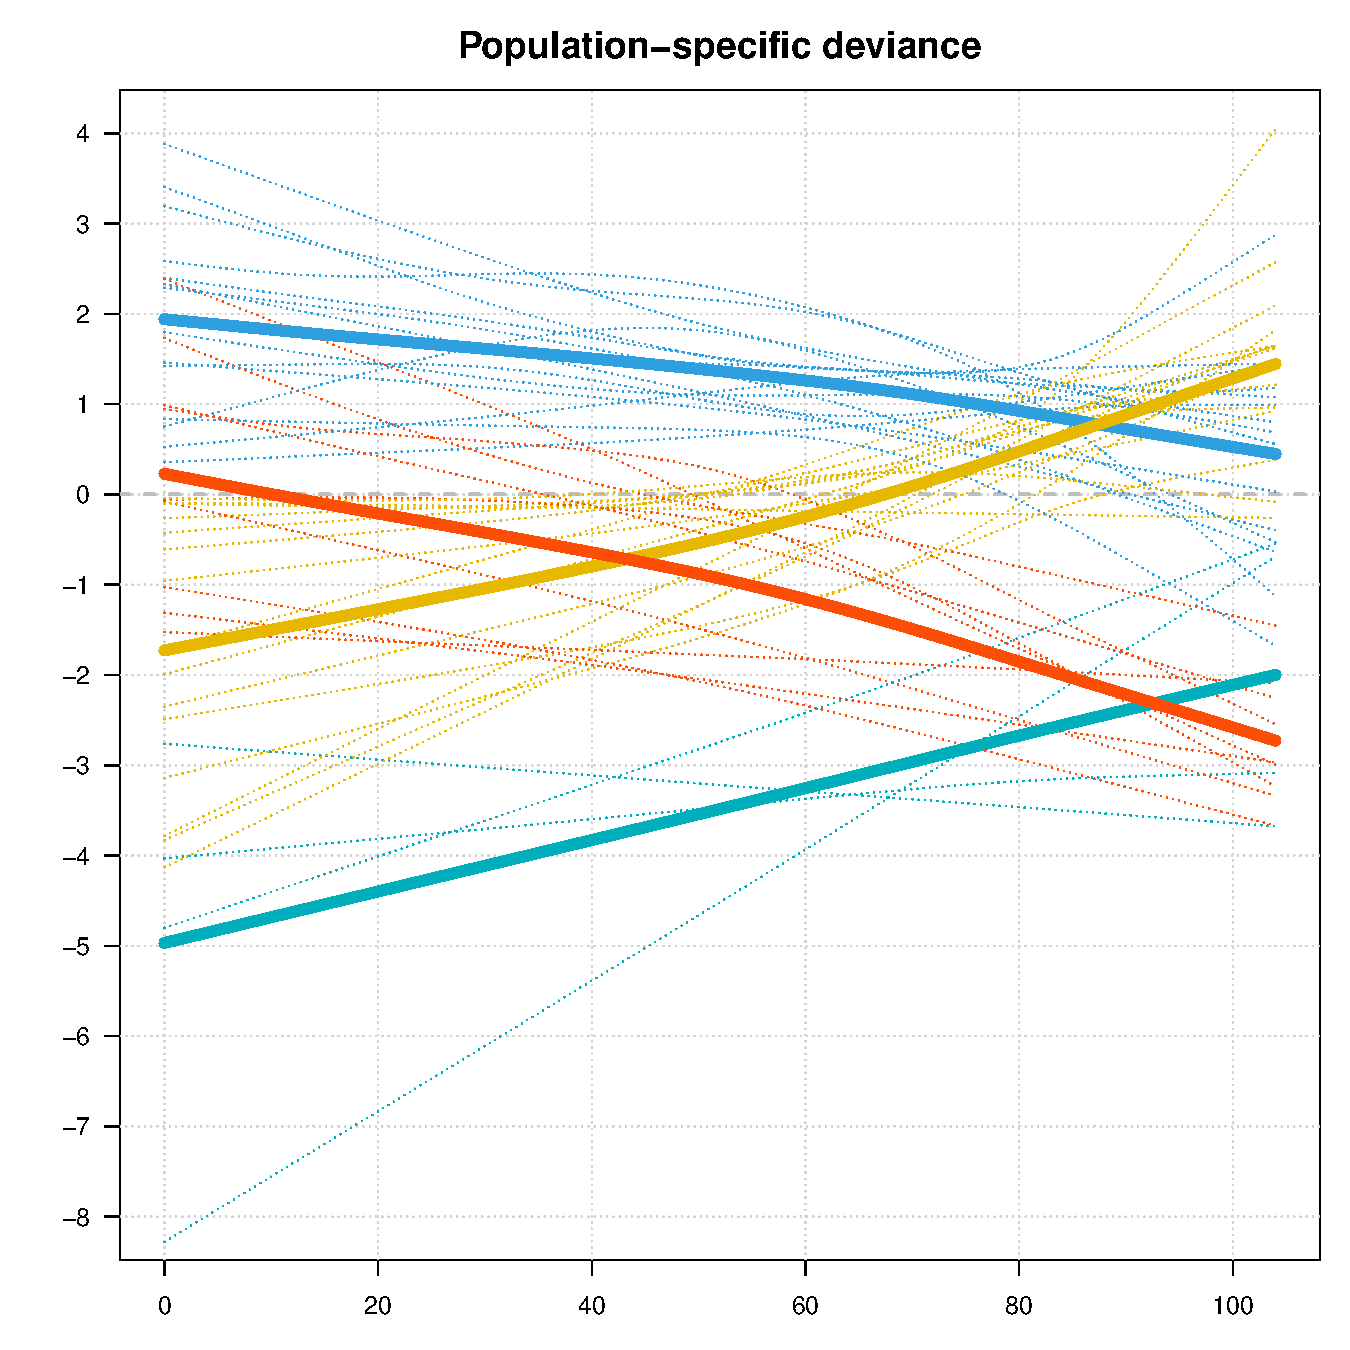
\includegraphics[scale=.23]{Figures/HierClust.pdf}
			\begin{tiny}
				Explained variance PC1+PC2: 77.3\% + 21.5\%
			\end{tiny}
		\end{column}
		\begin{column}{5cm}
			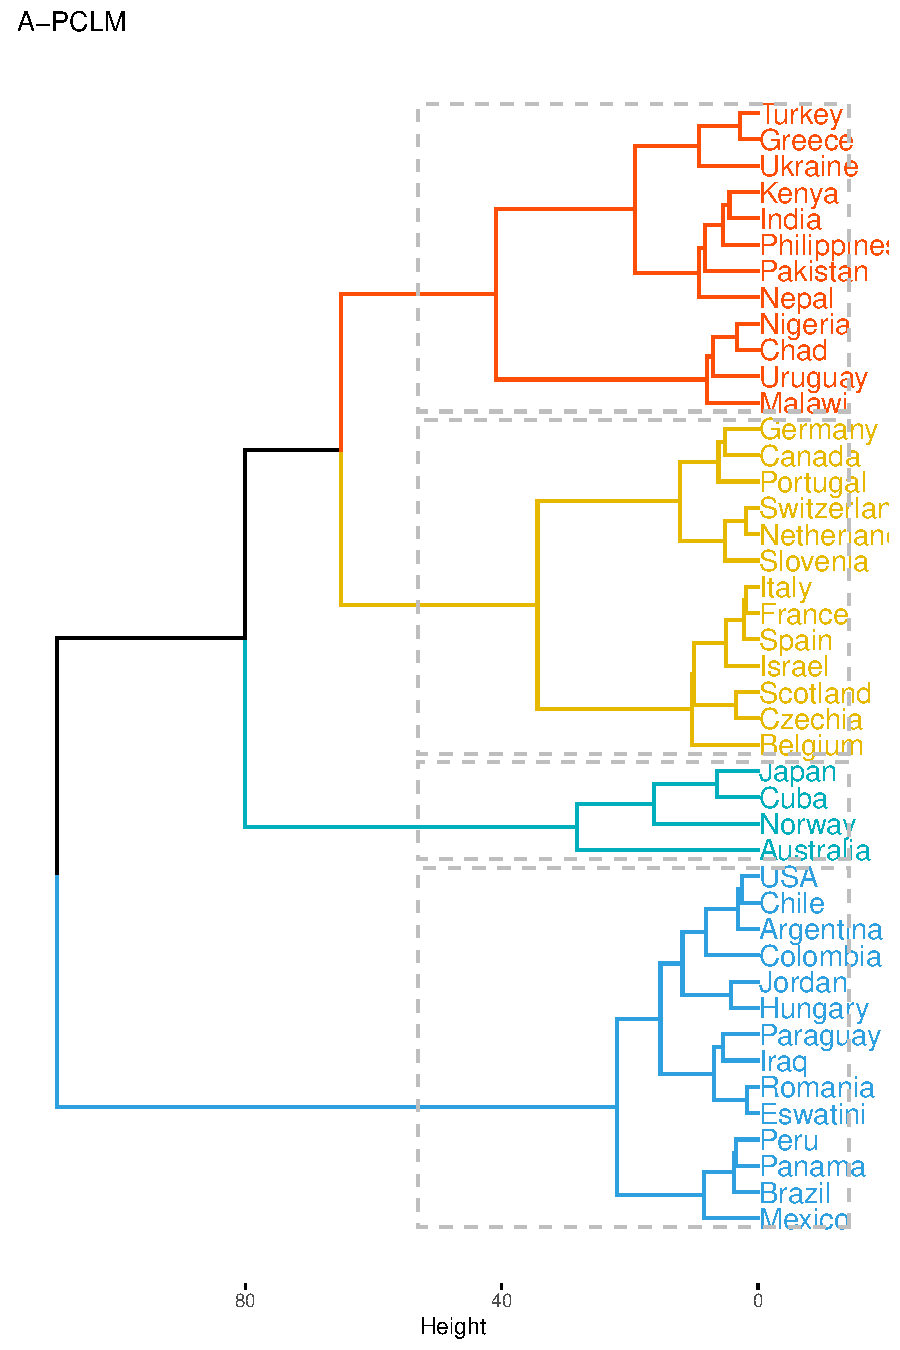
\includegraphics[scale=.35]{Figures/HierDendo.pdf}
		\end{column}
	\end{columns}
}
	\only<3>{
	\vspace{-0.5cm}
	\begin{center}
		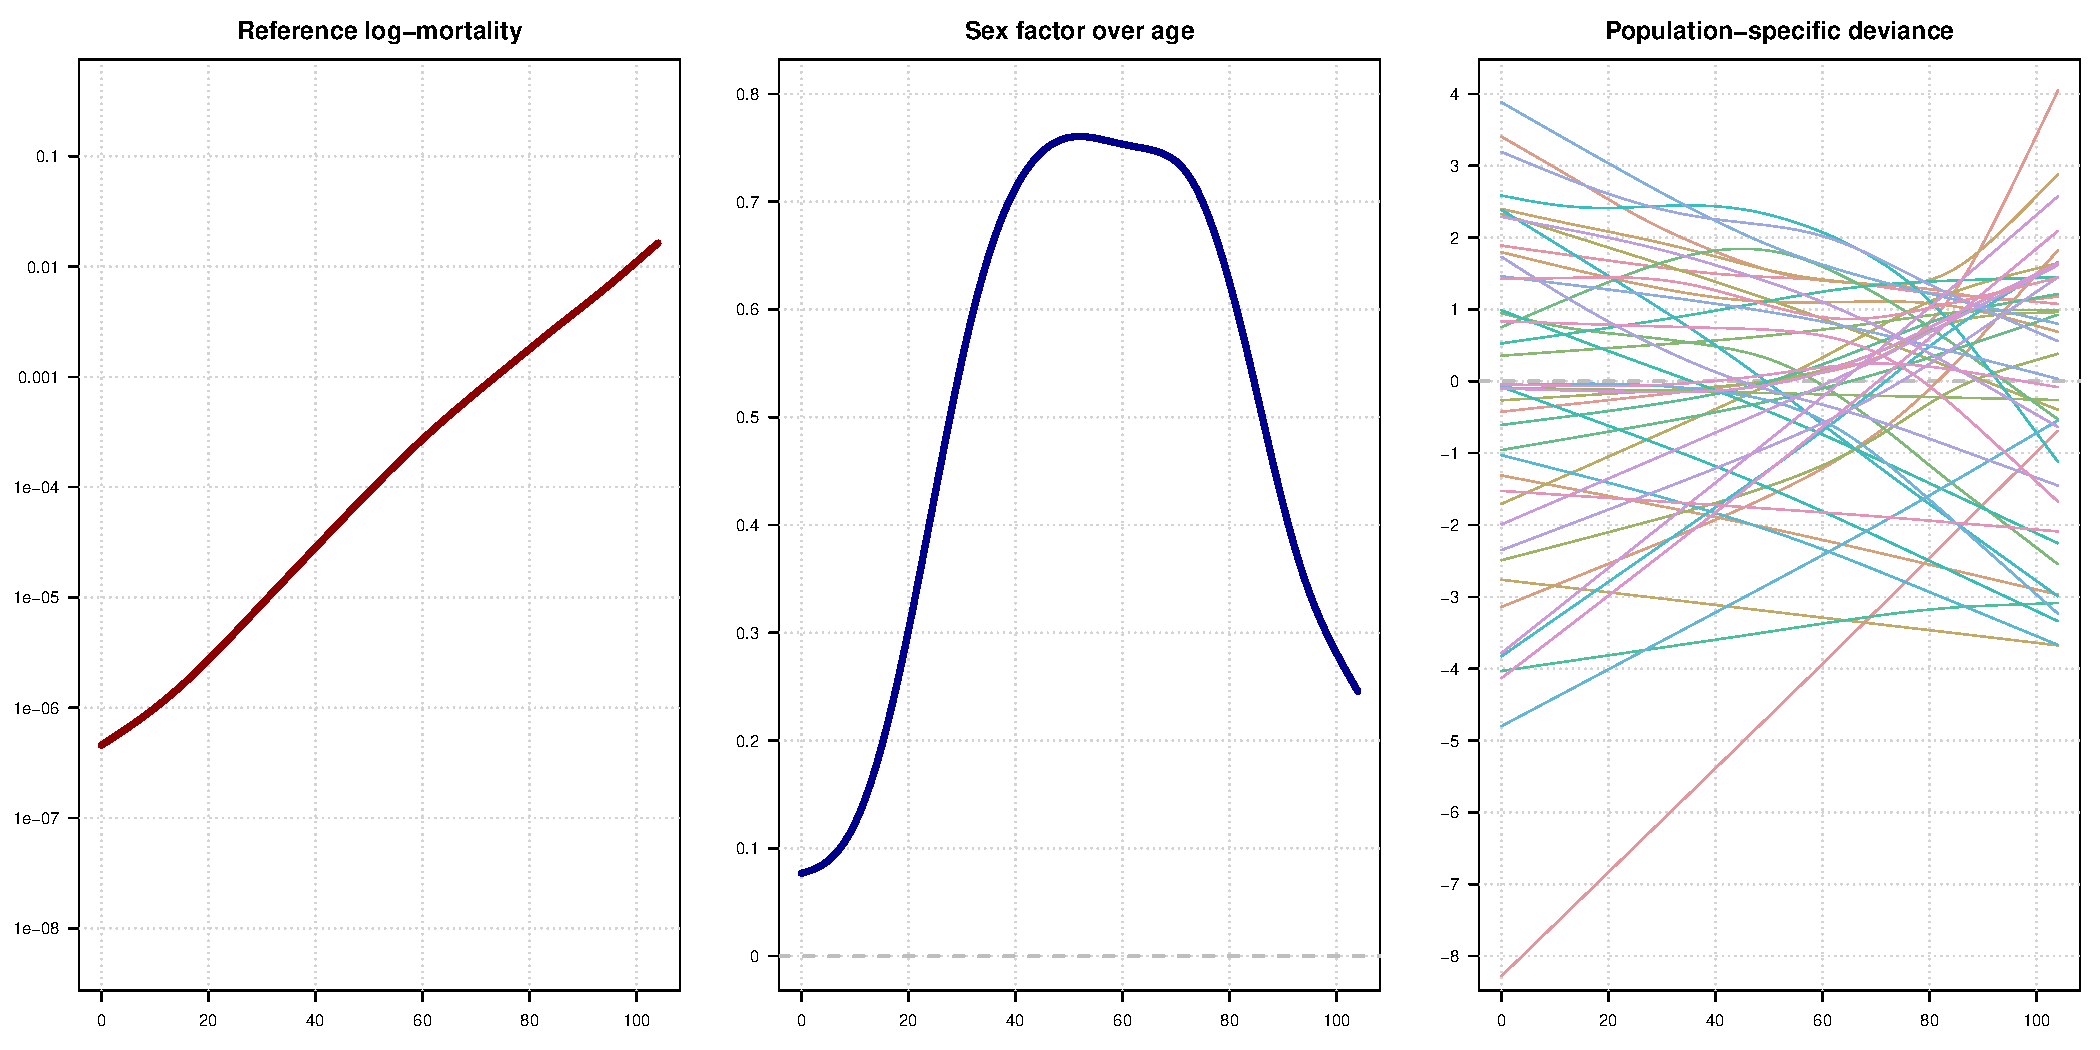
\includegraphics[scale=.2]{Figures/HierOut.pdf}% 77.3 + 21.5
		
		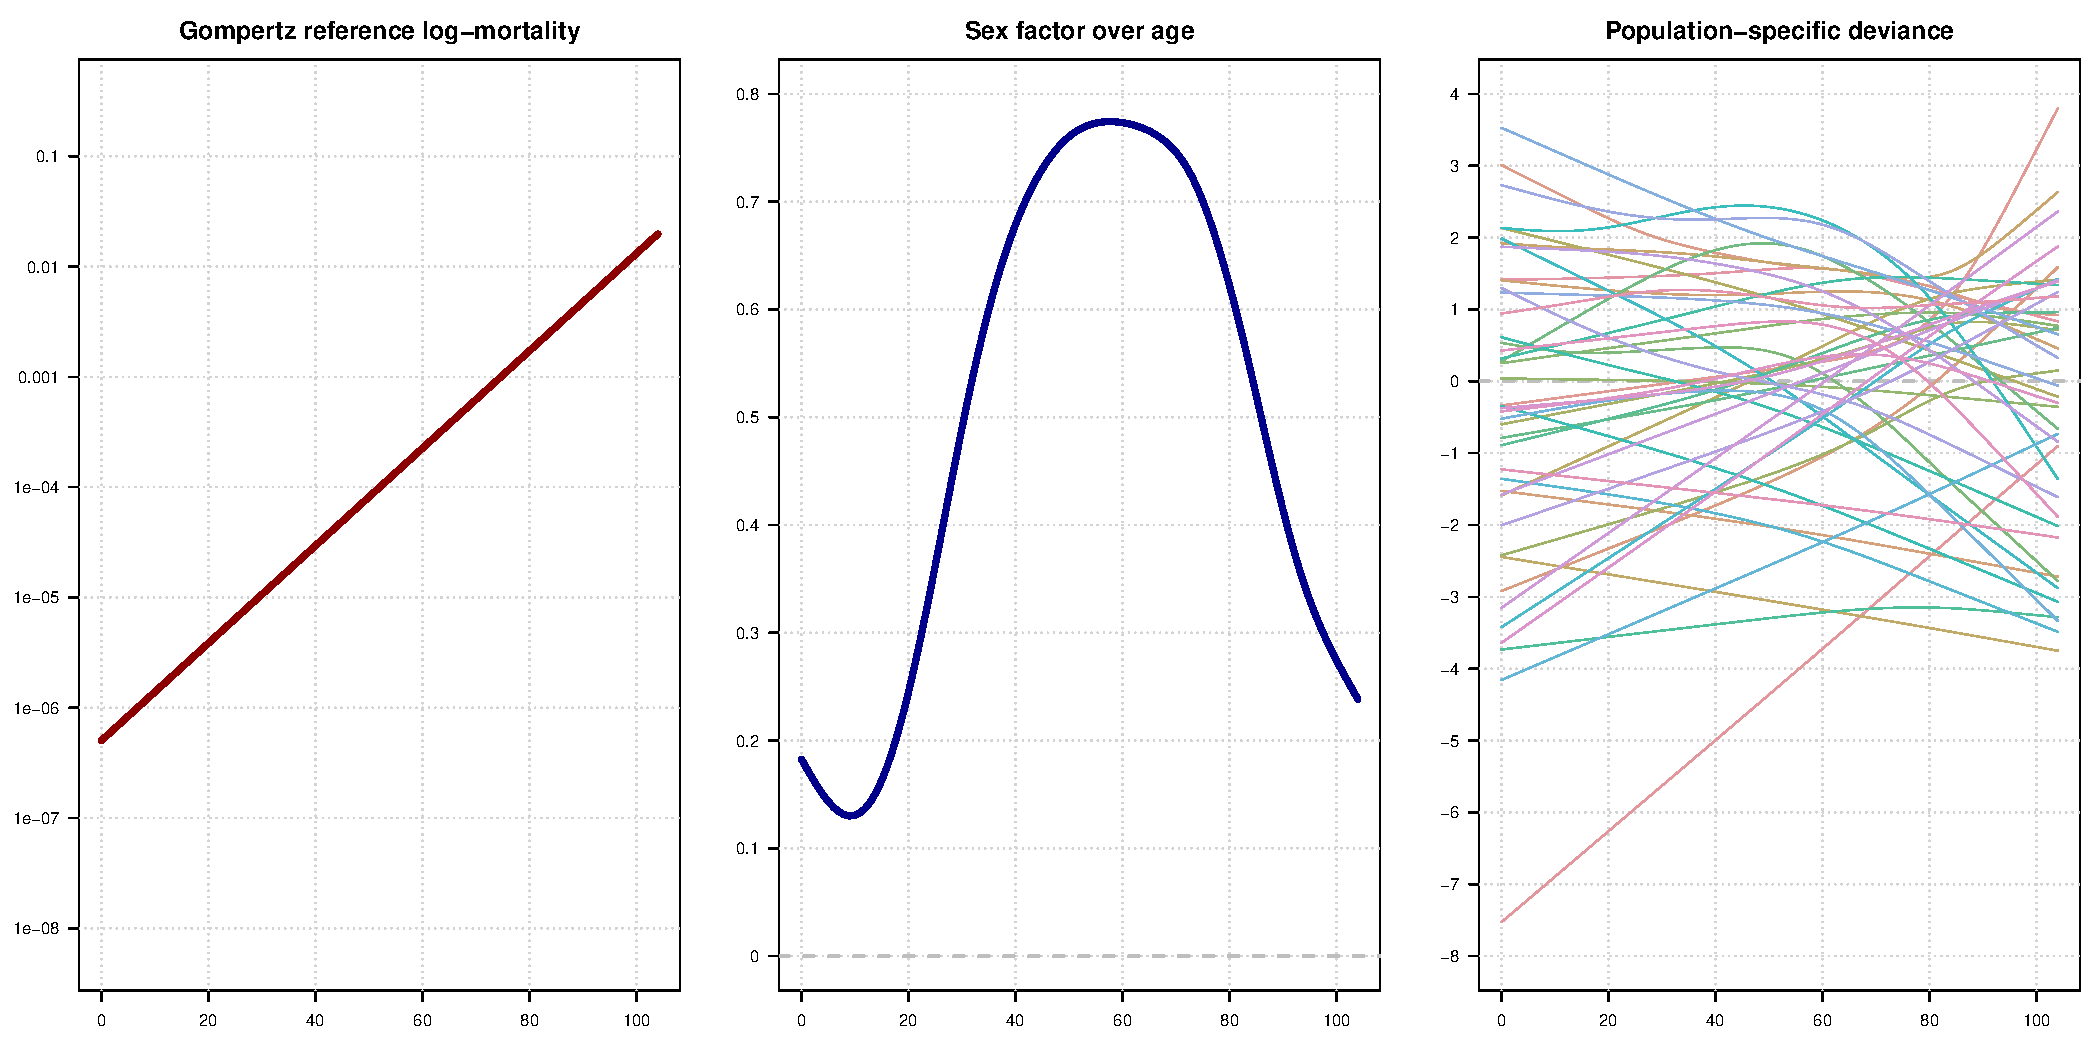
\includegraphics[scale=.2]{Figures/HierOutGomp.pdf}% 77.3 + 21.5
		
	\end{center}
}
	\only<4>{
	\begin{columns}
		\begin{column}{5cm}
			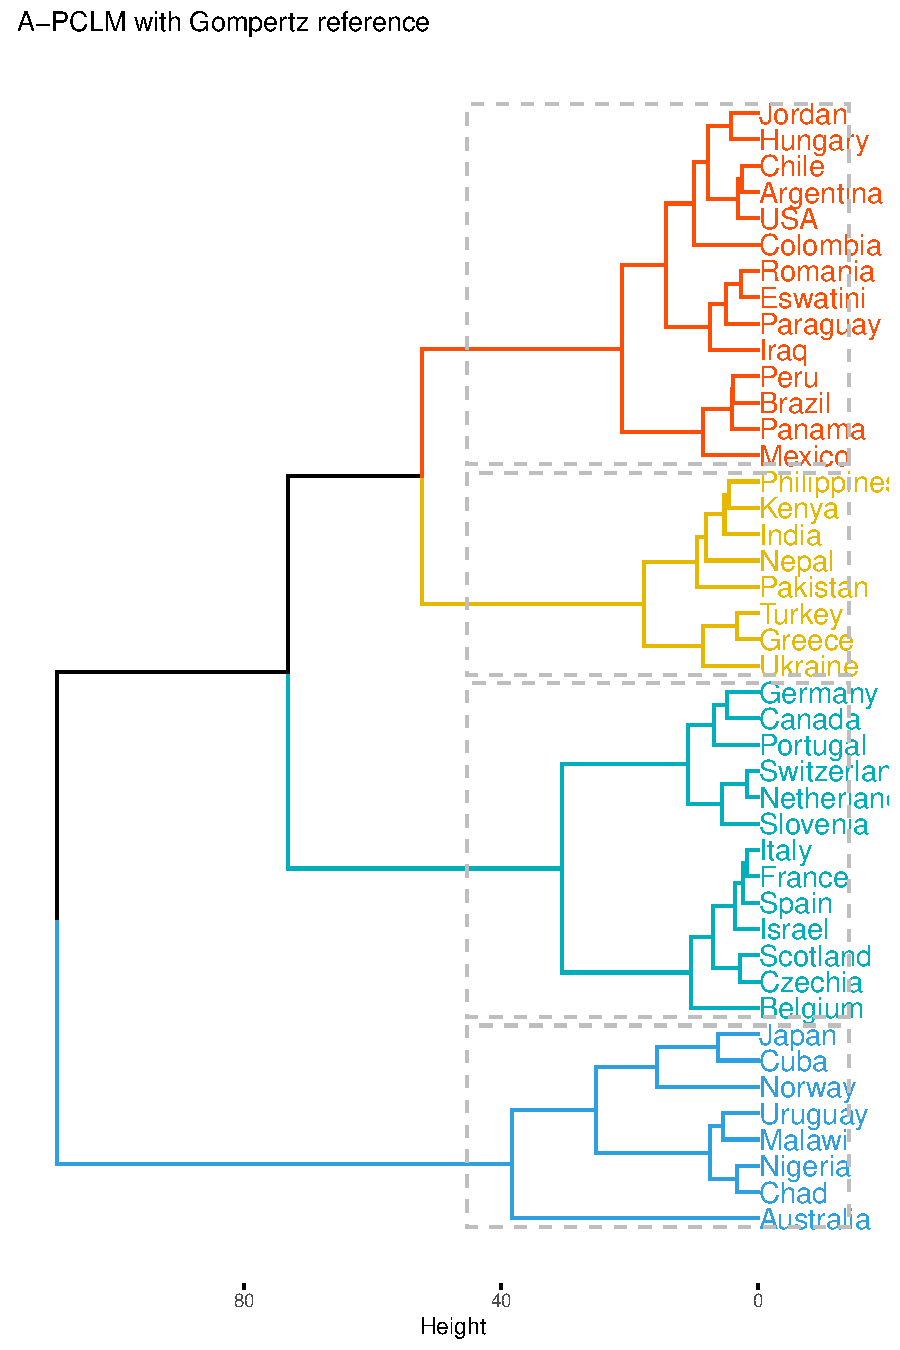
\includegraphics[scale=.35]{Figures/HierDendoGomp.pdf}
		\end{column}
		\begin{column}{5cm}
			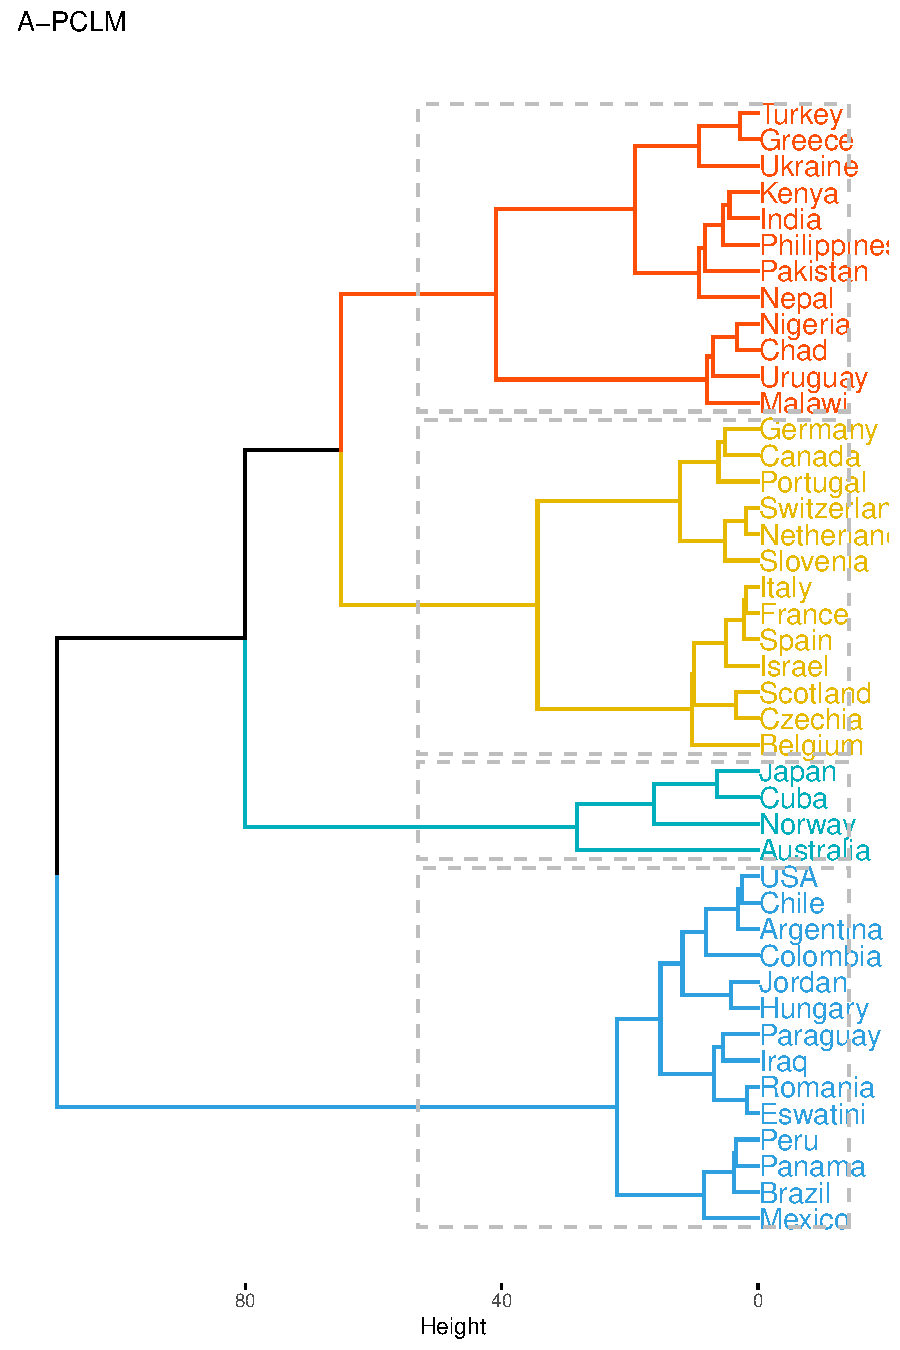
\includegraphics[scale=.35]{Figures/HierDendo.pdf}
		\end{column}
	\end{columns}
}
\end{frame}


\begin{frame}[fragile]\frametitle{Still to discuss/solve}
	\begin{itemize}
		\item \textbf{Main question}: What do we do when difference outcomes/models lead to different classification?
		\bigskip
		\item Unclear optimal number of clusters (fuzzy clustering?)
		\bigskip
		\item Restricting the analysis to adult mortality?
		\bigskip
		\item Mapping clusters to identify eventual (geographical) regions
		\bigskip
		\item ``Spatial borrowing'' to estimate when no data is available
		\bigskip
		\item Can we do the same exercise on excess mortality? Issue: data availability 
		\bigskip
		\item Computing confidence intervals of the estimates, optimizing smoothing parameters
\end{itemize}
\end{frame}

\end{document}


%%% -----------------------------------------------------  %%
%%% -----------------------------------------------------  %%
%\begin{frame}[fragile]\frametitle{Quick overview onuthe used data}
%\vspace{-0.4cm}
%\begin{columns}
%	\begin{column}{3.2cm}
%		\begin{itemize}
%			\item[]<1-> Age-specific death rates (probabilities)
%		\end{itemize}
%	\end{column}
%	\begin{column}{9.5cm}
%		\begin{footnotesize}
%			\begin{itemize}
%				\setlength\itemsep{0.1em}
%				\gooditem[\textbf{+}] standard tools for describing mortality (time-to-event)
%				\item[\textbf{+}] easy to incorporate stochasticity of the phenomenon
%				\pooritem[\textbf{--}] latest longevity processes may be missed
%			\end{itemize}
%		\end{footnotesize}
%	\end{column}
%\end{columns}
%\medskip
%\begin{columns}
%	\begin{column}{3.2cm}
%		\begin{itemize}
%			\item[]<2-> Age-at-death distributions
%		\end{itemize}
%	\end{column}
%	\begin{column}{9.5cm}
%		\onslide<2->{
%			\begin{footnotesize}
%				\begin{itemize}
%					\setlength\itemsep{0.1em}
%					\gooditem[\textbf{+}] latest longevity processes can be described
%					\item[\textbf{+}] alternative interpretations ($\sim$ AFT models)
%					\pooritem[\textbf{--}] often applicable only for adult ages
%				\end{itemize}
%			\end{footnotesize}
%		}
%	\end{column}
%\end{columns}
%\medskip
%\begin{columns}
%	\begin{column}{3.2cm}
%		\begin{itemize}
%			\item[]<3-> Survival improvement
%		\end{itemize}
%	\end{column}
%	\begin{column}{9.5cm}
%		\onslide<3->{
%			\begin{footnotesize}
%				\begin{itemize}
%					\setlength\itemsep{0.1em}
%					\gooditem[\textbf{+}] exploit regularities in mortality derivatives  	
%					\pooritem[\textbf{--}] prior model od the original data necessary
%					\item[\textbf{--}] difficulties in including uncertainty measures
%				\end{itemize}
%			\end{footnotesize}
%		}
%	\end{column}
%\end{columns}
%\medskip
%\begin{columns}
%	\begin{column}{3.2cm}
%		\begin{itemize}
%			\item[]<4-> Summary measures
%		\end{itemize}
%	\end{column}
%	\begin{column}{9.5cm}
%		\onslide<4->{
%			\begin{footnotesize}
%				\begin{itemize}
%					\setlength\itemsep{0.1em}
%					\gooditem[\textbf{+}] straightforward interpretation
%					\item[\textbf{+}] easy to impose prior assumptions
%					\pooritem[\textbf{--}] hard to move to complete age-time mortality profiles
%				\end{itemize}
%			\end{footnotesize}
%		}
%	\end{column}
%\end{columns}
%
%
%\end{frame}
%
%
%
%
%
%\begin{frame}[fragile]\frametitle{Placing some reference}
%
%\vspace{-1cm}
%{\fontsize{6pt}{9}\selectfont 
%	\begin{tabular}{p{8cm}p{0.5\textwidth}}
%		&
%		\begin{itemize}
%			\itemsep-0.3em 
%			\item[] {\color{Blue}Single population}
%			\item[] {\color{Green}More populations}
%			\item[] {\color{Red}Strata of population}
%		\end{itemize} 
%	\end{tabular}
%	\vspace{-1cm}
%	%\begin{tiny}
%	\begin{table}[]
%		\setlength\tabcolsep{1pt}
%		\hspace*{-0.8cm} 
%		\begin{tabular}{ccllll}
%			\multicolumn{2}{l}{} & \multicolumn{4}{c}{Data} \\ \cline{3-6} 
%			\multicolumn{2}{l|}{} & \multicolumn{1}{c|}{Rates/Probabilities} & \multicolumn{1}{c|}{Age-at-death distributions} & \multicolumn{1}{c|}{Rates-of-change} & \multicolumn{1}{c}{Summary measures} \\ \cline{2-6}
%			\multicolumn{1}{c|}{} & \multicolumn{1}{c|}{\cellcolor[HTML]{C0C0C0}Parametric} & \multicolumn{1}{l|}{\cellcolor[HTML]{C0C0C0}\begin{tabular}[c]{@{}l@{}}{\color{Blue}Classic models (1825-)}\\ {\color{Blue}Cairn et al. (2006)}\\ {\color{Red}Alai et al. (2018)}\end{tabular}} & \multicolumn{1}{l|}{\cellcolor[HTML]{C0C0C0}{\color{Blue}Janseen \& De Beer (2016)}} & \multicolumn{1}{l|}{\cellcolor[HTML]{C0C0C0}{\color{Blue}Haberman \& Renshaw (2012)}} & \cellcolor[HTML]{C0C0C0}{\color{Green}Raftery et al. (2013)} \\
%			\multicolumn{1}{c|}{} & \multicolumn{1}{l|}{\begin{tabular}[c]{@{}c@{}}Principal\\ component\end{tabular}} & \multicolumn{1}{l|}{\begin{tabular}[c]{@{}l@{}}{\color{Blue}Lee \& Carter (1992) + variants}\\ {\color{Green}Li \& Lee (2005)}\\ {\color{Red}Li et al. (2019)}\end{tabular}} & \multicolumn{1}{l|}{\begin{tabular}[c]{@{}l@{}}{\color{Red}Oeppen (2008)}\\ {\color{Green}Bergeron-Boucher et al. (2017)}\\ {\color{Red}Kj\ae rgaard et al. (2019)}\end{tabular}} & \multicolumn{1}{l|}{\begin{tabular}[c]{@{}l@{}}{\color{Blue}Mitchell et al. (2013)}\\ {\color{Green}Bohk \& Rau (2017)}\end{tabular}} &  \\
%			\multicolumn{1}{c|}{} & \multicolumn{1}{c|}{\cellcolor[HTML]{C0C0C0}Relational} & \multicolumn{1}{l|}{\cellcolor[HTML]{C0C0C0}{\color{Blue}De Beer (2012)}} & \multicolumn{1}{l|}{\cellcolor[HTML]{C0C0C0}{\color{Blue}Basellini \& Camarda (2019)}} & \multicolumn{1}{l|}{\cellcolor[HTML]{C0C0C0}} & \cellcolor[HTML]{C0C0C0}{\color{Blue}Torri \& Vaupel (2012)} \\
%			%		\rot{structure}&
%			\multicolumn{1}{c|}{\multirow{-8}{*}{\rotatebox[origin=c]{90}{structure}}} &
%			\multicolumn{1}{l|}{\begin{tabular}[c]{@{}c@{}}Non-\\ parametric\end{tabular}} & \multicolumn{1}{l|}{\begin{tabular}[c]{@{}l@{}}{\color{Blue}Currie et al. (2004)}\\ {\color{Blue}Camarda (2019)}\end{tabular}} & \multicolumn{1}{l|}{} & \multicolumn{1}{l|}{} & 
%		\end{tabular}
%	\end{table}
%}
%
%
%%\end{tiny} \parbox[t]{1mm}{\multirow{-7}{*}{\rotatebox[origin=c]{90}{structure}}}
%\end{frame}
%
%

%
%
%%
%%%% -----------------------------------------------------  %%
%%%% -----------------------------------------------------  %%
%%\begin{frame}[fragile]\frametitle{Outcomes from plain approaches}
%%\vspace{-0.1cm}
%%\begin{small}
%%  \begin{itemize}
%%\setlength\itemsep{0em}
%%  \item<1-> USA, males, ages 0-105, years 1960-2016, forecast years 2017-2050
%%  \end{itemize}
%%\end{small}
%%    \only<1>{
%%\vspace{-0.3cm}
%%      \begin{center}
%%        \includegraphics[scale=.30]{Figures/ExampleActualYEAR.pdf}
%%      \end{center}
%%    }
%%    \only<2>{
%%\vspace{-0.3cm}
%%      \begin{center}
%%        \includegraphics[scale=.30]{Figures/ExampleForecastYEAR.pdf}
%%      \end{center}
%%    }
%%\vspace{-0.2cm}
%%\begin{tiny}
%%\begin{itemize}
%%\setlength\itemsep{0em}
%%\item[] - Source: Human Mortality Database
%%\item[] - Delwarde et al.~(2007) for the smooth Lee-Carter
%%\item[] - Currie et al.~(2004) for the two-dimensional $P$-splines, 
%%\end{itemize}
%%
%%\end{tiny}
%%
%%\end{frame}
%%
%%\begin{frame}[fragile]\frametitle{The idea}
%%\begin{columns}
%%\begin{column}{5cm}
%%    \begin{block}{\textbf{$P$-splines:}}
%%\begin{itemize}
%%\gooditem flexibility (good fit)
%%\pooritem blind adherence extrapolation
%%\end{itemize}
%%    \end{block}
%%\end{column}
%%\begin{column}{5cm}
%%    \begin{block}{\textbf{Lee-Carter:}}
%%\begin{itemize}
%%\pooritem rigidity (bad fit)
%%\gooditem past development drives future mortality
%%\end{itemize}
%%    \end{block}
%%\end{column}
%%\end{columns}
%%\bigskip
%%\bigskip
%%\onslide<2->{
%%    \begin{alertblock}{\centering \textbf{Constrained $P$-splines, $CP$-splines:}}
%%Incorporate into $P$-splines demographic information
%%\begin{itemize}
%%\gooditem flexibility (good fit)
%%\gooditem future development based on prior demographic knowledge
%%\end{itemize}
%%\end{alertblock}
%%}
%%\end{frame}
%%
%\section[Lee-Carter]{The benchmark Lee-Carter model}
%
%\begin{frame}\frametitle{The model}
%\begin{itemize}
%	\item<1-> Lee and Carter (1992) suggested to model directly the
%	log-death rates:
%	\begin{equation*}
%	\ln(m_{ij}) =  {\color{Red}\alpha_{i}} +  {\color{Blue}\beta_{i}} \,  {\color{Green}\kappa_{j}} +
%	\epsilon_{ij}
%	\end{equation*}\begin{itemize}
%		\item ${\color{Red}\alpha_{i}}$, ${\color{Blue}\beta_{i}} $ and ${\color{Green}\kappa_{j}}$ are vectors of parameters
%		\item $\epsilon_{ij}$ is a matrix of errors
%	\end{itemize}
%	\medskip
%	\item<2-> Interpretation of the parameters:
%	\begin{itemize}
%		\item ${\color{Red}\alpha_{i}}$ is the general shape of the log-mortality at age $i$
%		\medskip
%		\item ${\color{Green}\kappa_{j}}$ represents the time trend
%		\medskip
%		\item ${\color{Blue}\beta_{i}}$ indicates the sensitivity of the log-mortality at age $i$ to
%		variations in the time index
%	\end{itemize}
%\end{itemize}
%\end{frame}
%
%%\begin{frame}\frametitle{Lee-Carter: schematic view}
%%\begin{small}
%%	\begin{itemize}
%%		\item<1->[]
%%		\begin{equation*}
%%		\left ( \begin{array}{cccc}
%%		\ln(m_{0,1960}) & \ln(m_{0,1961}) & \ldots & \ln(m_{0,2015})\\
%%		\ln(m_{1,1960}) & \ln(m_{1,1961}) & \ldots & \ln(m_{1,2015})\\
%%		\ln(m_{2,1960}) & \ln(m_{2,1961}) & \ldots & \ln(m_{2,2015})\\
%%		\vdots & \vdots & \ddots & \vdots \\
%%		\ln(m_{105,1960}) & \ln(m_{105,1961}) & \ldots & \ln(m_{105,2015})\\
%%		\end{array} \right ) \simeq
%%		\end{equation*}
%%		\begin{equation*}
%%		\left ( \begin{array}{c}
%%		{\color{Red}\alpha_{0}}\\
%%		{\color{Red}\alpha_{1}}\\
%%		{\color{Red}\alpha_{2}}\\
%%		{\color{Red}\vdots}\\
%%		{\color{Red}\alpha_{105}}\\
%%		\end{array} \right ) +
%%		\left ( \begin{array}{c}
%%		{\color{Blue}\beta_{0}}\\
%%		{\color{Blue}\beta_{1}}\\
%%		{\color{Blue}\beta_{2}}\\
%%		{\color{Blue}\vdots}\\
%%		{\color{Blue}\beta_{105}}\\
%%		\end{array} \right ) \,
%%		\left (
%%		\begin{array}{cccc}
%%		{\color{Green}\kappa_{1960}} & {\color{Green}\kappa_{1961}} & {\color{Green}\ldots} & {\color{Green}\kappa_{2015}}
%%		\end{array} \right )
%%		\end{equation*}
%%		\item<2->[]
%%		\begin{equation*}
%%		\underbrace{56}_{\mbox{years}} \times
%%		\underbrace{106}_{\mbox{ages}} = \underbrace{5936}_{\mbox{cells}}
%%		\simeq \underbrace{106}_{{\color{Red}\alpha_{i}}} + \underbrace{106}_{{\color{Blue}\beta_{i}}}
%%		+ \underbrace{56}_{{\color{Green}\kappa_{j}}} -
%%		\underbrace{2}_{\mbox{constraints}} = \underbrace{266}_{\mbox{parameters}}
%%		\end{equation*}
%%	\end{itemize}
%%\end{small}
%%\end{frame}
%
%\begin{frame}\frametitle{Estimation procedure}
%\begin{itemize}
%	\item<1-> Lee and Carter (1992) used Singular Value Decomposition
%%	\item<2-> Wilmoth (1993) suggested to fit the LC by Weighed Least-Squares (WLS)
%%	estimation
%	\item<2-> Brouhns et al.~(2002) suggested a Poisson log-bilinear model
%	for the estimated the LC
%
%\begin{itemize}
%\item Data: deaths and exposures over age and years: $Y_{ij}$ and $E_{ij}$
%\item Assumption: $Y_{ij} \sim \mathcal{P}(\mu_{ij} E_{ij})$ with $\mu_{ij} = \exp({\color{Red}\alpha_{i}} + {\color{Blue}\beta_{i}} \cdot {\color{Green}\kappa_{j}})$
%\item Maximization of the likelihood:
%$$
%\ln\mathcal{L}\left({\color{Red}\bm{\alpha}}, {\color{Blue}\bm{\beta}}, {\color{Green}\bm{\kappa}} | \, \bm{Y} , \bm{E}\right) \propto \sum_{i,j} \left[ Y_{ij} \, \ln \left ( \mu_{ij}  \right ) - E_{ij}\, \mu_{ij} \right]  \, . 
%$$
%\end{itemize}
%	\item<3-> Delwarde et al.~(2007) used penalized likelihood to enforce smoothness of parameter vectors:
%	\begin{small}
%	$$
%	\ln\mathcal{L}^{P}\left(\cdot\right) = \ln\mathcal{L}\left(\cdot\right) - \frac{1}{2} \,\lambda_{\alpha} \, {\color{Red}\bm{\alpha}}' \,\bm{D}'\bm{D} \, {\color{Red}\bm{\alpha}} - \frac{1}{2} \,\lambda_{\beta} \, {\color{Blue}\bm{\beta}}' \,\bm{D}'\bm{D} \, {\color{Blue}\bm{\beta}}
%	$$
%	\end{small}where $\lambda_{\alpha}$ and $\lambda_{\beta}$ control smoothness of ${\color{Red}\bm{\alpha}}$ and ${\color{Blue}\bm{\beta}}$ and $\bm{D}$ is the second order difference matrix
%\end{itemize}
%\end{frame}
%
%
%\begin{frame}[fragile]\frametitle{Portuguese female mortality in the light of Lee-Carter}
%\vspace{-0.4cm}
%\only<1>{
%	\begin{center}
%		\includegraphics[scale=.19]{Figures/LCalpha.pdf}
%		\includegraphics[scale=.19]{Figures/LCbeta.pdf}
%		\includegraphics[scale=.19]{Figures/LCkappa.pdf}
%	\end{center}
%}
%\end{frame}
%
%
%%\begin{frame}[fragile]\frametitle{Forecasting with the Lee-Carter}
%%\begin{itemize}
%%	\item Only ${\color{Green}\kappa_{j}}$ depends on time $\Rightarrow$ to forecast the whole surface:
%%	\begin{enumerate}
%%		\item fix ${\color{Red}\alpha_{i}}$ and ${\color{Blue}\beta_{i}}$
%%		\item extrapolate a single time-series (${\color{Green}\kappa_{j}}$), commonly rather linear
%%		\item given future ${\color{Green}\kappa_{j}}$, we reconstruct all age-year development
%%	\end{enumerate}
%%\bigskip
%%	\only<1>{
%%		
\includegraphics[scale=0.12]{./Figures/Empty}
%%	}
%%	\item<2-> Schematically:
%%\end{itemize}
%%\only<2>{
%%	\begin{small}
%%		\begin{equation*}
%%		\left ( \begin{array}{cccccc}
%%		\ln(m_{0,1960}) & \ldots & \ln(m_{0,2015}) \\
%%		\vdots  & \ddots & \vdots \\
%%		\ln(m_{105,1960}) & \ldots & \ln(m_{105,2015})\\
%%		\end{array} \right ) \simeq
%%		\end{equation*}
%%		\begin{equation*}
%%		\left ( \begin{array}{c}
%%		{\color{Red}\alpha_{0}}\\
%%		{\color{Red}\vdots}\\
%%		{\color{Red}\alpha_{105}}\\
%%		\end{array} \right ) +
%%		\left ( \begin{array}{c}
%%		{\color{Blue}\beta_{0}}\\
%%		{\color{Blue}\vdots}\\
%%		{\color{Blue}\beta_{105}}\\
%%		\end{array} \right ) \,
%%		\left (
%%		\begin{array}{ccc}
%%		{\color{Green}\kappa_{1960}} & {\color{Green}\ldots} & {\color{Green}\kappa_{2015}}
%%		\end{array} \right )
%%		\end{equation*}
%%	\end{small}
%%}
%%%
%%\only<3>{
%%	\begin{small}
%%		\begin{equation*}
%%		\left ( \begin{array}{cccccc}
%%		\ln(m_{0,1960}) & \ldots & \ln(m_{0,2015}) & {\color{orange}\ldots} & {\color{orange}\ldots} & {\color{orange}\ldots}\\
%%		\vdots  & \ddots & \vdots & {\color{orange}\vdots} & {\color{orange}\ddots} & {\color{orange}\vdots}\\
%%		\ln(m_{105,1960}) & \ldots & \ln(m_{105,2015})& {\color{orange}\ldots} & {\color{orange}\ldots} & {\color{orange}\ldots}\\
%%		\end{array} \right ) \simeq
%%		\end{equation*}
%%		\begin{equation*}
%%		\left ( \begin{array}{c}
%%		{\color{Red}\alpha_{0}}\\
%%		{\color{Red}\vdots}\\
%%		{\color{Red}\alpha_{105}}\\
%%		\end{array} \right ) +
%%		\left ( \begin{array}{c}
%%		{\color{Blue}\beta_{0}}\\
%%		{\color{Blue}\vdots}\\
%%		{\color{Blue}\beta_{105}}\\
%%		\end{array} \right ) \,
%%		\left (
%%		\begin{array}{cccccc}
%%		{\color{Green}\kappa_{1960}} & {\color{Green}\ldots} & {\color{Green}\kappa_{2015}} & {\color{orange}\kappa_{2016}} & {\color{orange}\ldots} & {\color{orange}\kappa_{2050}}
%%		\end{array} \right )
%%		\end{equation*}
%%	\end{small}
%%}	
%%\only<4>{
%%	\begin{small}
%%		\begin{equation*}
%%		\left ( \begin{array}{cccccc}
%%		\ln(m_{0,1960}) & \ldots & \ln(m_{0,2015}) & {\color{orange}\ln(m_{0,2016})} & {\color{orange}\ldots} & {\color{orange}\ln(m_{0,2050})}\\
%%		\vdots  & \ddots & \vdots & {\color{orange}\vdots} & {\color{orange}\ddots} & {\color{orange}\vdots}\\
%%		\ln(m_{105,1960}) & \ldots & \ln(m_{105,2015})& {\color{orange}\ln(m_{105,2016})} & {\color{orange}\ldots} & {\color{orange}\ln(m_{105,2050})}\\
%%		\end{array} \right ) \simeq
%%		\end{equation*}
%%		\begin{equation*}
%%		\left ( \begin{array}{c}
%%		{\color{Red}\alpha_{0}}\\
%%		{\color{Red}\vdots}\\
%%		{\color{Red}\alpha_{105}}\\
%%		\end{array} \right ) +
%%		\left ( \begin{array}{c}
%%		{\color{Blue}\beta_{0}}\\
%%		{\color{Blue}\vdots}\\
%%		{\color{Blue}\beta_{105}}\\
%%		\end{array} \right ) \,
%%		\left (
%%		\begin{array}{cccccc}
%%		{\color{Green}\kappa_{1960}} & {\color{Green}\ldots} & {\color{Green}\kappa_{2015}} & {\color{orange}\kappa_{2016}} & {\color{orange}\ldots} & {\color{orange}\kappa_{2050}}
%%		\end{array} \right )
%%		\end{equation*}
%%	\end{small}
%%}	
%%\end{frame}
%
%\begin{frame}[fragile]\frametitle{Future Portuguese female mortality \only<1,2>{: Lee-Carter ${\color{Green}\kappa_{j}}$}\only<3,4>{: log-rates}}
%\vspace{-0.1cm}
%\only<1>{
%	\begin{center}
%		\includegraphics[scale=.26]{Figures/LCkappaFor0.pdf}
%	\end{center}
%}
%\only<2>{
%	\begin{center}
%		\includegraphics[scale=.26]{Figures/LCkappaFor.pdf}
%	\end{center}
%}
%\only<3>{
%	\vspace{-0.4cm}
%	\begin{center}
%		\includegraphics[scale=.32]{Figures/ExampleLCYEAR.pdf}
%	\end{center}
%}
%\only<4>{
%	\vspace{-0.4cm}
%	\begin{center}
%		\includegraphics[scale=.32]{Figures/ExampleLCforYEAR.pdf}
%	\end{center}
%}
%\end{frame}
%
%\begin{frame}[fragile]\frametitle{Much more about the Lee-Carter}
%\begin{itemize}
%	\item Issues and solutions:
%	\medskip
%	
%	\begin{tabular}{ll}
%		Fix $\beta_{i}$: & {\scriptsize Li et al. (2013)}\\
%		Smoothness: &  {\scriptsize Hyndman and Ullah (2007); Currie (2014)}\\
%		Accounting for uncertainty: & {\scriptsize Brouhns et al. (2005); Koissi et al. (2006)}
%	\end{tabular}
%
%\bigskip
%\item Extensions:
%\medskip
%
%\begin{tabular}{ll}
%	Low quality data: & {\scriptsize Li et al. (2007)}\\
%More time-indexes: & {\scriptsize Hyndman and Ullah (2007)}\\
%Coherent forecast: & {\scriptsize Li and Lee (2005); Hyndman et al. (2013)}\\
%Cohort effects: & {\scriptsize Renshaw and Haberman (2006)}\\
%Bayesian estimation: & {\scriptsize Czado et al. (2005); Girosi and King (2008)}\\
%Age-pattern decomposition: & {\scriptsize Camarda and Basellini (2020)}
%\end{tabular}
%
%\end{itemize}
%
%
%\end{frame}
%
%
%\section[A non-parametric approach$\qquad\qquad$]{The statistical alternative: a non-parametric approach}
%
%%\begin{frame}[fragile]\frametitle{Data structure \& basic model}
%%\vspace{-0.5cm}
%%\begin{columns}
%%\begin{column}{0.5\textwidth}
%%%\vspace{-0.5cm}
%%\begin{center}
%%{\color{Blue}Observed data}\\\medskip
%%\includegraphics[scale=.2]{Figures/DataMort.pdf}
%%%        \includegraphics[scale=.2]{Figures/SchemeDEA.pdf}
%%%        \includegraphics[scale=.04]{Figures/SchemeWHITE.pdf}
%%%        \includegraphics[scale=.2]{Figures/SchemeEXP.pdf}
%%\end{center}
%%\onslide<2->{
%%	\vspace{-0.2cm}
%%\centering {\color{Green}Assumption:}
%%\vspace{-0.4cm}
%%$$
%%y_{ij} \sim \mathcal{P}(e_{ij} \,\mu_{ij})\, 
%%$$
%%}
%%\end{column}
%%% \vrule{}
%%\begin{column}{0.65\textwidth}
%%% \vspace{1cm}
%%\onslide<3->{
%%\centering{\color{Red}Model:}
%%}
%%\begin{itemize}
%%\setlength\itemsep{0em}
%%\item<3->[] $\bm{y} = \verb"vec"(\bm{Y})$
%%\item<3->[] $\bm{e} = \verb"vec"(\bm{E})$
%%\end{itemize}
%%\onslide<3->{
%%\vspace{-0.3cm}
%%\begin{eqnarray*}
%%\ln(\bm{y}) = \ln(\bm{e})+ \ln(\bm{\mu}) &=& \ln(\bm{e}) + \bm{\eta}\\
%%&=& \ln(\bm{e}) + \bm{B}\,\bm{\alpha}
%%\end{eqnarray*}
%%}
%%\vspace{-.7cm}
%%\begin{itemize}
%%\setlength\itemsep{0em}
%%\item<3->[] $\bm{B} = {\color{Blue}\bm{B}_{t_{1}}} \otimes {\color{Blue}\bm{B}_{a}}$
%%\item<3->[] $\bm{\alpha}$: penalized coefficients
%%\end{itemize}
%%\onslide<4->{
%%%\vspace{-.2cm}
%%\includegraphics[scale=.35]{Figures/KronBsplinesINK.pdf}
%%}
%%\end{column}
%%\end{columns}
%%\begin{small}
%%\vspace{-.5cm}
%%\begin{itemize}
%%\setlength\itemsep{0em}
%%\item<5-> estimated by a penalized iterative weighted least-squares algorithm
%%\end{itemize}
%%\end{small}
%%
%%\end{frame}
%
%
%
%\begin{frame}[fragile]\frametitle{Forecasting with $P$-splines (a missing value problem)}
%\begin{columns}
%	\begin{column}{4cm}
%		$\ln(\bm{y}) = \ln(\bm{e}) + \bm{B}\,\bm{\alpha}$
%	\end{column}
%	\begin{column}{5cm}
%\vspace{-.7cm}
%\begin{itemize}
%	\setlength\itemsep{0em}
%	\item<1->[] $\bm{B} = {\color{Blue}\bm{B}_{t_{1}}} \otimes {\color{Blue}\bm{B}_{a}}$
%	\item<1->[] $\bm{\alpha}$: penalized coefficients
%\end{itemize}
%\end{column}
%
%\end{columns}
%
%\smallskip
%\begin{itemize}
%\item<2-> Data are augmented with arbitrary future values and we define a weight matrix (Currie et al.~2004)
%\item<3-> $B$-spline bases are augmented too: $\bm{B} = [{\color{Blue}\bm{B}_{t_{1}}}:{\color{Red}\bm{B}_{t_{2}}}] \otimes {\color{Blue}\bm{B}_{a}}$
%\end{itemize}
%\begin{itemize}
%\pooritem<4-> No information about mortality structure is used
%\end{itemize}
%
%\begin{columns}
%\begin{column}{0.55\textwidth}
%\onslide<2->{
%\includegraphics[scale=.12]{Figures/SchemeDEAfor.pdf}
%        % \includegraphics[scale=.02]{Figures/SchemeWHITE.pdf}
%\includegraphics[scale=.12]{Figures/SchemeEXPfor.pdf}
%        % \includegraphics[scale=.02]{Figures/SchemeWHITE.pdf}
%\includegraphics[scale=.12]{Figures/SchemeWEIfor.pdf}
%}
%\end{column}
%\begin{column}{0.6\textwidth}
%\only<1,2>{\includegraphics[scale=.4]{Figures/KronBsplinesINK.pdf}}
%\only<3->{\includegraphics[scale=.4]{Figures/KronBsplinesFORINK.pdf}}
%\end{column}
%\end{columns}
%
%
%\end{frame}
%%
%%% -----------------------------------------------------  %%
%%% -----------------------------------------------------  %%
%%\section{$CP$-splines}
%%
%%%% -----------------------------------------------------  %%
%%%% -----------------------------------------------------  %%
%\begin{frame}\frametitle{Observing mortality patterns (over ages)}
%\vspace{-0.3cm}
%\begin{itemize}
%\item<1-> Over ages we observe certain regularities in mortality shape
%\vspace{0.3cm}
%\only<1>{
%	\begin{center}
%\includegraphics[scale=.24]{Figures/ExampleAgeShape.pdf}
%\includegraphics[scale=.24]{Figures/ExampleAgeDerivEmpty.pdf}
%\end{center}
%}
%\only<2>{
%	\begin{center}
%\includegraphics[scale=.24]{Figures/ExampleAgeShape.pdf}
%\includegraphics[scale=.24]{Figures/ExampleAgeDeriv.pdf}
%\end{center}
%}
%\vspace{0.1cm}
%\item<2-> Interested solely in shapes (regardless their levels), these
%regularities are condensed in the (relative) derivatives
%\end{itemize}
%\end{frame}
%
%%% -----------------------------------------------------  %%
%%% -----------------------------------------------------  %%
%\begin{frame}[fragile]\frametitle{Observing mortality patterns (over years)}
%\vspace{-0.3cm}
%  \begin{itemize}
%  \item<1-> Variations over time are larger than over age
%  \item<2-> We can still observe regularities for each age
%\only<1>{
%		\begin{center}
%        \includegraphics[scale=.18]{Figures/EmptyYear.pdf}
%
%        \includegraphics[scale=.18]{Figures/EmptyYear.pdf}
%        	\end{center}
%    }
%\only<2>{
%		\begin{center}
%        \includegraphics[scale=.18]{Figures/ExampleYearShape.pdf}
%
%        \includegraphics[scale=.18]{Figures/EmptyYear.pdf}
%                	\end{center}
%    }
%\only<3>{
%		\begin{center}
%        \includegraphics[scale=.18]{Figures/ExampleYearShape1.pdf}
%
%        \includegraphics[scale=.18]{Figures/ExampleYearDeriv.pdf}
%                	\end{center}
%    }
%\only<4>{
%		\begin{center}
%        \includegraphics[scale=.18]{Figures/ExampleYearShape1.pdf}
%
%        \includegraphics[scale=.18]{Figures/ExampleYearDerivCI.pdf}
%                	\end{center}
%    }
%\only<5>{
%		\begin{center}
%\includegraphics[scale=.36]{Figures/ExampleYearDerivCIallAges.pdf}       
%        	\end{center}
%    }
%\item<3-> Interested in age-specific rate-of-change,
%  i.e.~derivatives
%\item<4-> Ignore small fluctuations $\Rightarrow$ we take 50\%
%  confidence interval 
%\end{itemize}
%
%\end{frame}
%
%
% \begin{frame}[fragile]\frametitle{Working on the shape}
% \begin{itemize}
% \item<1-> Disregarding information about shapes seems unreasonable
% \medskip
% \item<2-> Future mortality {\color{Red}\emph{must}} follow data-driven
%   age-profiles and rate-of-change
% \medskip
% \item<3-> We constrain derivatives of future mortality to lay
%   within certain confidence intervals of observed derivatives
% \medskip
% \item<4-> Asymmetric penalties are employed for this purpose:
% \begin{itemize}
% % \item the main idea behind this penalty lays in its local behavior 
% \item within each iteration, whenever current estimations present
%   derivatives (in future years) out of the desired intervals, a
%   penalty intervenes 
% \end{itemize}
% \end{itemize}
%  \onslide<5->{
%  \begin{block}{}
%  	\centering 	\color{Red}{\begin{Large}
%  			$CP$-splines 
%  		\end{Large}} 
%  \end{block}	
%\smallskip
%
%{\scriptsize
%Camarda, C. G. (2019).\\
%Smooth Constrained Mortality Forecasting. \\
%\textit{Demographic Research}. \textbf{41} (38), 1091-1130\\
%}
%}
% \end{frame}
%
%
%
%\begin{frame}[fragile]\frametitle{Future Portuguese female mortality by both approaches}\vspace{-0.1cm}
%\only<1>{
%	\vspace{-0.4cm}
%	\begin{center}
%		\includegraphics[scale=.32]{Figures/ExampleLCCPSforYEAR.pdf}
%	\end{center}
%}
%\only<2>{
%	\vspace{-0.4cm}
%	\begin{center}
%		\includegraphics[scale=.26]{Figures/ExampleE0.pdf}
%		\includegraphics[scale=.26]{Figures/ExampleEDink.pdf}
%	\end{center}
%}
%\only<3>{
%	\begin{center}
%		\animategraphics[autoplay,scale=0.21]{5}{./Figures/ExampleLCforAGEanim}{0}{90}
%		\animategraphics[autoplay,scale=0.21]{5}{./Figures/ExampleCPSforAGEanim}{0}{90}
%	\end{center}
%}
%
%\end{frame}
%
%
%\section*{$\qquad$}
%
%
%
%\begin{frame}[fragile]\frametitle{Take-home messages}
%%\begin{itemize}
%%	\item<1-> blabla
%%\end{itemize}
%\onslide<1->{
%	\begin{block}{\centering \color{Blue}{\textbf{Conclusion:}}}
%		\centering  
%		\color{Red}{\begin{large}
%				Despite its well deserved success, the Lee-Carter model has 
%				\begin{itemize}
%					\item monopolized the field
%					\item intrinsic flaws, which are only partially solved
%				\end{itemize}
%			\end{large}
%		}
%	\end{block}
%}
%\bigskip
%\onslide<2->{
%	\begin{block}{\centering \color{Blue}{\textbf{Corollary:}}}
%		\centering  
%		\color{Red}{\begin{large}
%		New paradigms are necessary \\(are non-parametric approaches possible avenues?)\\
%			\end{large}
%		}
%	\end{block}
%}
%\end{frame}
%
%
%\begin{frame}\frametitle{$\,$}
%\vspace{-0.5cm}
%{\color{Red}
%\begin{center}
%	\begin{tabular}{lll}
%		$\qquad$$\qquad$$\qquad$$\qquad$ $\qquad$$\qquad$&
%		$\qquad$ \\  
%		\hline
%	\end{tabular}
%\end{center}
%}
%
%%
%\begin{center}
%\begin{LARGE}
%	Thanks for your attention.\\
%	\smallskip
%	Comments and questions?
%\end{LARGE}
%\end{center}
%\vspace{-0.7cm}
%{\color{Red}
%\begin{center}
%	\begin{tabular}{lll}
%		$\qquad$$\qquad$$\qquad$$\qquad$ $\qquad$$\qquad$&
%		$\qquad$ \\  
%		\hline
%	\end{tabular}
%\end{center}
%}
%\begin{center}
%\begin{large}
%	\smallskip
%	
%	%\texttt{carlo-giovanni.camarda@ined.fr}\\
%	
%	{\color{Blue}\texttt{sites.google.com/site/carlogiovannicamarda}}
%	
%	
%	\bigskip
%	\bigskip
%	\bigskip
%	
%	
%\end{large}
%\end{center}
%%
%%\begin{tiny}
%%\epigraph{\emph{Null hypothesis is never proved or established, \\but is possibly disproved, \\in the course of experimentation.}}{Ronald Fisher (1935)\\\emph{The Design of Experiments} \\Oliver and Boyd, p.~18}
%%\end{tiny}
%
%\end{frame}
%
%
%
%
%%
%%
%%
%%
%%\section{$P$-spline intermezzo}
%%
%%
%%\begin{frame}\frametitle{Simple least-squares}
%%\begin{itemize}
%%	\item<1-> We have an $n$-vector $\bm{y}$ and covariate(s) $\bm{x}$
%%	\item<2-> We assume $E(y_{i}) = \mu_{i} = \alpha_{0} + \alpha_{1} x_{i}$
%%	\item<3-> We minimize:
%%	\begin{eqnarray*}
%%		S = \sum_{i=1}^{n} \left[ y_{i} - ({\color{Red}\alpha_{0}} + {\color{Green}\alpha_{1} x_{i}}\only<6->{+ {\color{Blue}\alpha_{2} x^{2}_{i}}}\only<7->{+ {\color{Cyan}\alpha_{3} x^{3}_{i}}}\only<8->{+ {\color{violet}\alpha_{4} x^{4}_{i}}})\right]^{2}
%%	\end{eqnarray*}
%%	\item<4-> In matrix:
%%	\onslide<4,5>{
%%		\begin{eqnarray*}
%%			\bm{X} = \left[ \begin{array}{cc}
%%				{\color{Red}1} & {\color{Green}x_{1}} \\
%%				{\color{Red}1} & {\color{Green}x_{2}} \\
%%				{\color{Red}\vdots} & {\color{Green}\vdots} \\
%%				{\color{Red}1} & {\color{Green}x_{n}} \\
%%			\end{array}\right]
%%			\quad \bm{\alpha} = \left[ \begin{array}{c}
%%				{\color{Red}\alpha_{0}} \\
%%				{\color{Green}\alpha_{1}} \\
%%			\end{array}\right]
%%			\quad \bm{\mu} = \bm{X} \bm{\alpha}
%%		\end{eqnarray*}
%%	}
%%	\vspace{-2.5cm}
%%	\onslide<6>{
%%		\begin{eqnarray*} \bm{X} = \left[ \begin{array}{ccc}
%%				{\color{Red}1} & {\color{Green}x_{1}} & {\color{Blue}x^{2}_{1}}\\
%%				{\color{Red}1} & {\color{Green}x_{2}} & {\color{Blue}x^{2}_{2}}\\
%%				{\color{Red}\vdots} & {\color{Green}\vdots} & {\color{Blue}\vdots} \\
%%				{\color{Red}1} & {\color{Green}x_{n}} & {\color{Blue}x^{2}_{n}}
%%			\end{array}\right]
%%			\quad \bm{\alpha} = \left[ \begin{array}{c}
%%				{\color{Red}\alpha_{0}} \\
%%				{\color{Green}\alpha_{1}} \\
%%				{\color{Blue}\alpha_{2}}
%%			\end{array}\right]
%%			\quad , \quad \bm{\mu} = \bm{X} \bm{\alpha}
%%		\end{eqnarray*}
%%	}
%%	\vspace{-2.5cm}
%%	\onslide<7>{
%%		\begin{eqnarray*} \bm{X} = \left[ \begin{array}{cccc}
%%				{\color{Red}1} & {\color{Green}x_{1}} & {\color{Blue}x^{2}_{1}} & {\color{Cyan}x^{3}_{1}}\\
%%				{\color{Red}1} & {\color{Green}x_{2}} & {\color{Blue}x^{2}_{2}} & {\color{Cyan}x^{3}_{2}}\\
%%				{\color{Red}\vdots} & {\color{Green}\vdots} & {\color{Blue}\vdots} & {\color{Cyan}\vdots}\\
%%				{\color{Red}1} & {\color{Green}x_{n}} & {\color{Blue}x^{2}_{n}} & {\color{Cyan}x^{3}_{n}}\\
%%			\end{array}\right]
%%			\quad \bm{\alpha} = \left[ \begin{array}{c}
%%				{\color{Red}\alpha_{0}} \\
%%				{\color{Green}\alpha_{1}} \\
%%				{\color{Blue}\alpha_{2}} \\
%%				{\color{Cyan}\alpha_{3}}
%%			\end{array}\right]
%%			\quad , \quad \bm{\mu} = \bm{X} \bm{\alpha}
%%		\end{eqnarray*}
%%	}
%%	\vspace{-2.5cm}\onslide<8>{
%%		\begin{eqnarray*} \bm{X} = \left[ \begin{array}{ccccc}
%%				{\color{Red}1} & {\color{Green}x_{1}} & {\color{Blue}x^{2}_{1}} & {\color{Cyan}x^{3}_{1}} & {\color{violet}x^{4}_{1}}\\
%%				{\color{Red}1} & {\color{Green}x_{2}} & {\color{Blue}x^{2}_{2}} & {\color{Cyan}x^{3}_{2}} & {\color{violet}x^{4}_{2}}\\
%%				{\color{Red}\vdots} & {\color{Green}\vdots} & {\color{Blue}\vdots}  & {\color{Cyan}\vdots} & {\color{violet}\vdots}   \\
%%				{\color{Red}1} & {\color{Green}x_{n}} & {\color{Blue}x^{2}_{n}} & {\color{Cyan}x^{3}_{n}} & {\color{violet}x^{4}_{n}}\\
%%			\end{array}\right]
%%			\quad \bm{\alpha} = \left[ \begin{array}{c}
%%				{\color{Red}\alpha_{0}} \\
%%				{\color{Green}\alpha_{1}} \\
%%				{\color{Blue}\alpha_{2}} \\
%%				{\color{Cyan}\alpha_{3}} \\
%%				{\color{violet}\alpha_{4}}
%%			\end{array}\right]
%%			\quad , \quad \bm{\mu} = \bm{X} \bm{\alpha}
%%		\end{eqnarray*}
%%	}
%%	
%%	\item<5-> We minimize: $|\bm{y} - \bm{X}\bm{\alpha}|^{2} \quad \Rightarrow \quad 
%%	\bm{X}'\bm{X}\bm{\alpha} = \bm{X}\bm{y} \quad \Rightarrow \quad 
%%	\hat{\bm{\alpha}} = (\bm{X}'\bm{X})^{-1} \bm{X}'\bm{y}$
%%\end{itemize}
%%\end{frame}
%%
%%
%%\begin{frame}\frametitle{Model matrices}
%%\vspace{-0.5cm}      
%%\only<1>{
%%\begin{figure}
%%	\begin{center}
%%		\includegraphics[scale=.47]{Figures/ModMat1.pdf}
%%	\end{center}
%%\end{figure}
%%} 
%%\only<2>{
%%\begin{figure}
%%	\begin{center}
%%		\includegraphics[scale=.47]{Figures/ModMat2.pdf}
%%	\end{center}
%%\end{figure}
%%}
%%\end{frame}
%%
%%
%%
%%\begin{frame}\frametitle{Can we do better?}
%%\begin{itemize}
%%\item<1->[]
%%\begin{itemize}
%%\item Simple basis is good for simple example
%%\medskip
%%\item Basis function (powers of $x$) are global
%%\medskip
%%\item Moving one end moves the other end too
%%\medskip
%%\item Unexpected wiggles
%%\medskip
%%\item The higher the degree the more is sensitive
%%\end{itemize}
%%\bigskip
%%\item<2->[]
%%\begin{itemize}
%%\item We seek for local basis
%%\medskip
%%\item Useful for more complex data
%%\medskip
%%\item No assumptions on the trend (let the data speak by themselves!)
%%\medskip
%%\item Smooth outcomes
%%\end{itemize}
%%\end{itemize}
%%\end{frame}
%%
%%\begin{frame}\frametitle{Slightly more complex example}
%%\vspace{-0.5cm}
%%\only<1>{
%%\begin{figure}
%%\begin{center}
%%\includegraphics[scale=.47]{Figures/SimData.pdf}
%%\end{center}
%%\end{figure}
%%}
%%\end{frame}
%%
%%
%%\begin{frame}\frametitle{Introducing $B$-splines}
%%\vspace{-0.2cm}
%%\begin{itemize}
%%\item<1-> Create a suitable basis $\Rightarrow$ (equidistant) $B$-splines:
%%\begin{footnotesize}
%%\begin{eqnarray*}
%%\bm{B} = \left[ \begin{array}{ccccc}
%%B_{1}(x_{1}) & B_{2}(x_{1}) & {\color<2->{Red}B_{3}(x_{1})}
%%& \ldots & B_{k}(x_{1})\\ 
%%B_{1}(x_{2}) & B_{2}(x_{2}) & {\color<2->{red}B_{3}(x_{2})}
%%& \ldots & B_{k}(x_{2})\\ 
%%\vdots & \vdots & {\color<2->{Red}\vdots} & \vdots & \vdots
%%\\ 
%%B_{1}(x_{n}) & B_{2}(x_{n}) & {\color<2->{Red}B_{3}(x_{n})}
%%& \ldots & B_{k}(x_{n})\\ 
%%\end{array}\right]
%%\end{eqnarray*}
%%\end{footnotesize}
%%%\vspace{-0.2cm}
%%\only<1>{
%%	\begin{figure}
%%		\begin{center}
%%\includegraphics[scale=.25]{Figures/SingleBsplEmpty.pdf}
%%		\end{center}
%%\end{figure}
%%}
%%\only<2>{\begin{figure}
%%\begin{center}
%%\includegraphics[scale=.25]{Figures/SingleBspl.pdf}
%%\end{center}
%%\end{figure}}
%%\only<3->{\begin{figure}
%%\begin{center}
%%\includegraphics[scale=.25]{Figures/BsplBases.pdf}
%%\end{center}
%%\end{figure}}
%%\item<4-> $E(\bm{y}) = \bm{\mu} = \bm{B}\,\bm{\alpha} \quad
%%\Rightarrow  \quad \hat{\bm{\alpha}} = (\bm{B}'\bm{B})^{-1}
%%\bm{B}'\bm{y}$ 
%%\end{itemize}
%%\end{frame}
%%
%%\begin{frame}\frametitle{Fitting with 20 $B$-splines}
%%\vspace{-0.5cm}
%%\only<1>{
%%\begin{center}
%%\includegraphics[scale=0.47]{Figures/DataBspl.pdf} 
%%\end{center}
%%}  
%%\only<2>{
%%\begin{center}
%%\includegraphics[scale=0.47]{Figures/DataBsplUnpen.pdf} 
%%\end{center}
%%}  
%%\end{frame}
%%
%%\begin{frame}\frametitle{Penalizing the coefficients: $P$-splines}
%%\begin{itemize}
%%\item<1-> Outcomes are not smooth, we could:
%%\begin{itemize}
%%\item take less $B$-splines
%%\item place each $B$-splines in specific positions
%%\item<2-> set a double goal:
%%\end{itemize}
%%\only<2->{
%%\begin{enumerate}
%%\item good fit to the data, i.e.~low least-squares: $S =
%%|\bm{y} - \bm{B}\bm{\alpha}|^{2}$ 
%%\item smooth curve, i.e.~low roughness: $R = |\bm{D}
%%\bm{\alpha}|^{2}$ 
%%\end{enumerate}
%%}
%%\item<3-> We balance this two object-functions:
%%\begin{eqnarray*}
%%S^{*} = S + \lambda R = |\bm{y} - \bm{B}\bm{\alpha}|^{2} +
%%\lambda |\bm{D} \bm{\alpha}|^{2}
%%\end{eqnarray*}
%%\item<4-> Given a $\lambda$, this is again a linear system of
%%equation with explicit solution: 
%%\begin{eqnarray*}
%%\hat{\bm{\alpha}} = (\bm{B}'\bm{B} + \lambda
%%\bm{D}'\bm{D})^{-1} \bm{B}'\bm{y}
%%\end{eqnarray*}
%%\end{itemize}
%%\end{frame}
%%
%%
%%\begin{frame}\frametitle{Including a penalty, $d=2$}
%%\vspace{-0.5cm}
%%\only<1>{
%%\begin{center}
%%\includegraphics[scale=0.47]{Figures/DataBspl.pdf} 
%%\end{center}
%%}  
%%\only<2>{
%%\begin{center}
%%\includegraphics[scale=0.47]{Figures/DataBsplUnpen.pdf} 
%%\end{center}
%%}  
%%\only<3>{
%%\begin{center}
%%\includegraphics[scale=0.47]{Figures/DataBsplPen.pdf} 
%%\end{center}
%%}  
%%\only<4>{
%%\begin{center}
%%\animategraphics[loop, autoplay, scale=0.47, palindrome]{5}{Figures/PenBsplAnim}{0}{12}
%%\end{center}
%%}
%%
%%\end{frame}
%%
%%
%%\begin{frame}\frametitle{$P$-splines for Poisson data}
%%\begin{itemize}
%%\item<1-> In demography we love counting $\Rightarrow$ $y_i \sim \mathcal{P}(\mu_{i})$ 
%%\medskip
%%\item<2-> We use a ``linear predictor'': $\bm{\eta} =\ln(\bm{\mu}) = \bm{B}\bm{\alpha}$ 
%%\medskip
%%\item<3-> We have a non-linear system of equations, in an iterative
%%process, at step $t+1$: 
%%\begin{eqnarray*}
%%\tilde{\bm{\alpha}}_{t+1} = (\bm{B}'\tilde{\bm{W}}_{t}\bm{B} + \lambda \bm{D}'\bm{D})^{-1}
%%\bm{B}'\hat{\bm{W}}_{t}\tilde{\bm{z}}_{t} \, ,
%%\end{eqnarray*}
%%where 
%%
%%$\tilde{\bm{z}} = (\bm{y} - \tilde{\bm{\mu}}) /
%%\tilde{\bm{\mu}} + \bm{B}\tilde{\bm{\alpha}}$ (working dependent variable)
%%
%%\medskip
%%
%%$\tilde{\bm{W}} = diag(\tilde{\bm{\mu}})$ (weight matrix)
%%\bigskip
%%\item<4-> We can include an offset (exposures for mortality data)
%%just changing: 
%%\begin{eqnarray*}
%%\bm{\mu} = \bm{e} \, \exp(\bm{\eta}) = \exp(\bm{B}\bm{\alpha} +
%%\ln(\bm{e}))
%%\end{eqnarray*}
%%\end{itemize}
%%\end{frame}
%%
%%
%%
%%\section{$P$-splines for forecasting}
%%
%%\begin{frame}[fragile]\frametitle{Data structure \& basic model}
%%% \vspace{-1cm}
%%\begin{columns}
%%\begin{column}{0.5\textwidth}
%%\vspace{-0.5cm}
%%\begin{center}
%%{\color{Blue}Observed data}\\\medskip
%%        \includegraphics[scale=.2]{Figures/SchemeDEA.pdf}
%%        \includegraphics[scale=.04]{Figures/SchemeWHITE.pdf}
%%        \includegraphics[scale=.2]{Figures/SchemeEXP.pdf}
%%\end{center}
%%\onslide<2->{
%%\centering {\color{Green}Assumption:}
%%$$
%%y_{ij} \sim \mathcal{P}(e_{ij} \,\mu_{ij})\, 
%%$$
%%}
%%\end{column}
%%% \vrule{}
%%\begin{column}{0.7\textwidth}
%%% \vspace{1cm}
%%\onslide<3->{
%%\centering{\color{Red}Model:}
%%}
%%\begin{itemize}
%%\setlength\itemsep{0em}
%%\item<3->[] $\bm{y} = \verb"vec"(\bm{Y})$
%%\item<3->[] $\bm{e} = \verb"vec"(\bm{E})$
%%\end{itemize}
%%\onslide<3->{
%%\vspace{-0.3cm}
%%\begin{eqnarray*}
%%\ln(\bm{y}) = \ln(\bm{e})+ \ln(\bm{\mu}) &=& \ln(\bm{e}) + \bm{\eta}\\
%%&=& \ln(\bm{e}) + \bm{B}\,\bm{\alpha}
%%\end{eqnarray*}
%%}
%%\vspace{-.7cm}
%%\begin{itemize}
%%\setlength\itemsep{0em}
%%\item<3->[] $\bm{B} = {\color{Blue}\bm{B}_{t_{1}}} \otimes {\color{Blue}\bm{B}_{a}}$
%%\item<3->[] $\bm{\alpha}$: penalized coefficients
%%\end{itemize}
%%\onslide<4->{
%%%\vspace{-.2cm}
%%\includegraphics[scale=.35]{Figures/KronBsplinesINK.pdf}
%%}
%%\end{column}
%%\end{columns}
%%\begin{small}
%%\vspace{-.1cm}
%%\begin{itemize}
%%\setlength\itemsep{0em}
%%\item<5-> estimated by a penalized iterative weighted least-squares algorithm
%%\end{itemize}
%%\end{small}
%%
%%\end{frame}
%%
%%
%%
%%\begin{frame}[fragile]\frametitle{Forecasting with $P$-splines}
%%\begin{itemize}
%%\item<1-> Forecasting is treated as a missing value problem
%%\item<2-> Data are augmented with arbitrary future values and we define a weight matrix
%%\item<3-> $B$-spline bases are augmented too: $\bm{B} = [{\color{Blue}\bm{B}_{t_{1}}}:{\color{Red}\bm{B}_{t_{2}}}] \otimes {\color{Blue}\bm{B}_{a}}$
%%\item<4-> The original algorithm can be adapted
%%\end{itemize}
%%\begin{itemize}
%%\pooritem<5-> No information about mortality structure is used
%%\end{itemize}
%%
%%\onslide<2->{
%%\begin{columns}
%%\begin{column}{0.55\textwidth}
%%\includegraphics[scale=.12]{Figures/SchemeDEAfor.pdf}
%%        % \includegraphics[scale=.02]{Figures/SchemeWHITE.pdf}
%%\includegraphics[scale=.12]{Figures/SchemeEXPfor.pdf}
%%        % \includegraphics[scale=.02]{Figures/SchemeWHITE.pdf}
%%\includegraphics[scale=.12]{Figures/SchemeWEIfor.pdf}
%%\end{column}
%%\begin{column}{0.6\textwidth}
%%\onslide<3->{\includegraphics[scale=.4]{Figures/KronBsplinesFORINK.pdf}}}
%%\end{column}
%%\end{columns}
%%
%%
%%\end{frame}
%%
%%% -----------------------------------------------------  %%
%%% -----------------------------------------------------  %%
%%\section{$CP$-splines}
%%
%%%% -----------------------------------------------------  %%
%%%% -----------------------------------------------------  %%
%%\begin{frame}\frametitle{Observing mortality patterns (over ages)}
%%\vspace{-0.3cm}
%%\begin{itemize}
%%\item<1-> Over ages we observe certain regularities in mortality shape
%%\vspace{0.3cm}
%%\only<1>{
%%	\begin{center}
%%\includegraphics[scale=.24]{Figures/UsaAgeShape.pdf}
%%\includegraphics[scale=.24]{Figures/UsaAgeDerivEmpty.pdf}
%%\end{center}
%%}
%%\only<2>{
%%	\begin{center}
%%\includegraphics[scale=.24]{Figures/UsaAgeShape.pdf}
%%\includegraphics[scale=.24]{Figures/UsaAgeDeriv.pdf}
%%\end{center}
%%}
%%\vspace{0.1cm}
%%\item<2-> Interested solely in shapes (regardless their levels), these
%%regularities are condensed in the (relative) derivatives
%%\end{itemize}
%%\end{frame}
%%
%%%% -----------------------------------------------------  %%
%%%% -----------------------------------------------------  %%
%%\begin{frame}[fragile]\frametitle{Observing mortality patterns (over years)}
%%\vspace{-0.3cm}
%%  \begin{itemize}
%%  \item<1-> Variations over time are larger than over age
%%  \item<2-> We can still observe regularities for each age
%%\only<1>{
%%		\begin{center}
%%        \includegraphics[scale=.18]{Figures/EmptyYear.pdf}
%%
%%        \includegraphics[scale=.18]{Figures/EmptyYear.pdf}
%%        	\end{center}
%%    }
%%\only<2>{
%%		\begin{center}
%%        \includegraphics[scale=.18]{Figures/UsaYearShape.pdf}
%%
%%        \includegraphics[scale=.18]{Figures/EmptyYear.pdf}
%%                	\end{center}
%%    }
%%\only<3>{
%%		\begin{center}
%%        \includegraphics[scale=.18]{Figures/UsaYearShape1.pdf}
%%
%%        \includegraphics[scale=.18]{Figures/UsaYearDeriv.pdf}
%%                	\end{center}
%%    }
%%\only<4>{
%%		\begin{center}
%%        \includegraphics[scale=.18]{Figures/UsaYearShape1.pdf}
%%
%%        \includegraphics[scale=.18]{Figures/UsaYearDerivCI.pdf}
%%                	\end{center}
%%    }
%%\only<5>{
%%		\begin{center}
%%\includegraphics[scale=.36]{Figures/UsaYearDerivCIallAges.pdf}       
%%        	\end{center}
%%    }
%%\item<3-> Interested in age-specific rate-of-change,
%%  i.e.~derivatives
%%\item<4-> Ignore small fluctuations $\Rightarrow$ we take 50\%
%%  confidence interval 
%%\end{itemize}
%%
%%\end{frame}
%%
%%
%% \begin{frame}[fragile]\frametitle{Working on the shape}
%% \begin{itemize}
%% \item<1-> Disregarding information about shapes seems unreasonable
%% \medskip
%% \item<2-> Future mortality {\color{Red}\emph{must}} follow data-driven
%%   age-profiles and rate-of-change
%% \medskip
%% \item<3-> We constrain derivatives of future mortality to lay
%%   within certain confidence intervals of observed derivatives
%% \medskip
%% \item<4-> Asymmetric penalties are employed for this purpose:
%% \begin{itemize}
%% % \item the main idea behind this penalty lays in its local behavior 
%% \item within each iteration, whenever current estimations present
%%   derivatives (in future years) out of the desired intervals, a
%%   penalty intervenes 
%% \end{itemize}
%% \medskip
%% \item<5> Let's see how it works in action for a specific year (2035) and a
%%   specific age (50)
%% \end{itemize}
%% \end{frame}
%%
%%\begin{frame}[fragile]\frametitle{Asymmetric penalty in action}
%%  \only<1>{
%%    \centering \textbf{Without} asymmetric penalty\\
%%%    \smallskip
%%%    \vspace{1.5cm}
%%%    \hspace{-0.5cm}
%%    \begin{center}
%%    \includegraphics[scale=.26]{Figures/NoAsyAder.pdf}
%%%    \includegraphics[scale=.01]{Figures/EmptyYear.pdf}
%%    \includegraphics[scale=.26]{Figures/NoAsyYderEmpty.pdf}
%%    \end{center}
%%  }
%%  \only<2>{
%%    \centering \textbf{Without} asymmetric penalty\\
%%%\smallskip
%%%    $\,$
%%%    \vspace{1.5cm}
%%%    \hspace{-0.5cm}
%%    \begin{center}
%%    \includegraphics[scale=.26]{Figures/NoAsyAder.pdf}
%% %   \includegraphics[scale=.01]{Figures/EmptyYear.pdf}
%%    \includegraphics[scale=.26]{Figures/NoAsyYder.pdf}
%%    \end{center}
%%  }
%%
%%  \only<3>{
%%	\centering \textbf{With} asymmetric penalty\\
%%	%\smallskip
%%	%    $\,$
%%	%    \vspace{1.5cm}
%%	%    \hspace{-0.5cm}
%%	\begin{center}
%%		\includegraphics[scale=.26]{Figures/AsyAder.pdf}
%%		%   \includegraphics[scale=.01]{Figures/EmptyYear.pdf}
%%		\includegraphics[scale=.26]{Figures/AsyYder.pdf}
%%	\end{center}
%%}
%%  \only<4>{
%%	\centering \textbf{With} asymmetric penalty\\
%%\smallskip
%%    \begin{center}
%%      \animategraphics[autoplay, scale=0.25, loop]{1}{./Figures/AnimLoop}{0}{14}
%%    \end{center}
%%  }
%%
%%\end{frame}
%%
%%
%%\section{Results}
%%
%%\begin{frame}[fragile]\frametitle{Outcomes for US, males}
%%
%%    \only<1>{
%%\vspace{-0.5cm}
%%      \begin{center}
%%        \includegraphics[scale=.32]{Figures/OutcomesUsaYEAR.pdf}
%%\begin{footnotesize}
%%Log-mortality. Ages 0-105, observed years 1960-2016, forecast up to 2050 
%%\end{footnotesize}
%%      \end{center}
%%    }
%%    \only<2>{
%%\vspace{-0.5cm}
%%      \begin{center}
%%        \includegraphics[scale=.32]{Figures/OutcomesUsaAGE.pdf}
%%\begin{footnotesize}
%%Log-mortality. Ages 0-105, observed years 1960-2016, forecast up to 2050 
%%\end{footnotesize}
%%      \end{center}
%%
%%    }
%%  \only<3>{
%%\vspace{-0.5cm}
%%      \begin{center}
%%        \includegraphics[scale=.26]{Figures/OutcomesUsaLE.pdf}
%%        \includegraphics[scale=.26]{Figures/UsaAgeDerivEmpty.pdf}
%%\smallskip
%%
%%\begin{footnotesize}
%%Life Expectancy. \\Ages 0-105, observed years 1960-2016, forecast up to 2050 
%%\end{footnotesize}
%%      \end{center}
%%  }
%%  \only<4>{
%%\vspace{-0.5cm}
%%      \begin{center}
%%        \includegraphics[scale=.26]{Figures/OutcomesUsaLE.pdf}
%%        \includegraphics[scale=.26]{Figures/OutcomesUsaEDINK.pdf}
%%\smallskip
%%
%%\begin{footnotesize}
%%Life Expectancy and Lifespan variability measure
%%($e_{0}^{\dagger}$). \\Ages 0-105, observed years 1960-2016, forecast
%%up to 2050  
%%\end{footnotesize}
%%      \end{center}
%%  }
%%
%%\end{frame}
%%
%%
%%\begin{frame}[fragile]\frametitle{Outcomes for Denmark, females}
%%
%%    \only<1>{
%%\vspace{-0.5cm}
%%      \begin{center}
%%        \includegraphics[scale=.32]{Figures/OutcomesDnkYEAR.pdf}
%%\begin{footnotesize}
%%Log-mortality. Ages 0-105, observed years 1960-2016, forecast up to 2050 
%%\end{footnotesize}
%%      \end{center}
%%    }
%%    \only<2>{
%%\vspace{-0.5cm}
%%      \begin{center}
%%        \includegraphics[scale=.32]{Figures/OutcomesDnkAGE.pdf}
%%\begin{footnotesize}
%%Log-mortality. Ages 0-105, observed years 1960-2016, forecast up to 2050 
%%\end{footnotesize}
%%      \end{center}
%%
%%    }
%%  \only<3>{
%%\vspace{-0.5cm}
%%      \begin{center}
%%        \includegraphics[scale=.26]{Figures/OutcomesDnkLE.pdf}
%%        \includegraphics[scale=.26]{Figures/UsaAgeDerivEmpty.pdf}
%%\smallskip
%%
%%\begin{footnotesize}
%%Life Expectancy. \\Ages 0-105, observed years 1960-2016, forecast up to 2050 
%%\end{footnotesize}
%%      \end{center}
%%  }
%%  \only<4>{
%%\vspace{-0.5cm}
%%      \begin{center}
%%        \includegraphics[scale=.26]{Figures/OutcomesDnkLE.pdf}
%%        \includegraphics[scale=.26]{Figures/OutcomesDnkEDINK.pdf}
%%\smallskip
%%
%%\begin{footnotesize}
%%Life Expectancy and Lifespan variability measure
%%($e_{0}^{\dagger}$). \\Ages 0-105, observed years 1960-2016, forecast
%%up to 2050  
%%\end{footnotesize}
%%      \end{center}
%%  }
%%
%%\end{frame}
%%
%%\section{Conclusions}
%%
%%
%%\begin{frame}[fragile]\frametitle{What I haven't shown here, $\ldots$}
%%\begin{itemize}
%%	\item[]<1->
%%	\begin{itemize}
%%		\item All associated equations
%%		\medskip
%%		\item How we address infant mortality in a smoothing setting
%%		\medskip
%%		\item Bootstrap procedure to obtain confidence interval
%%		\medskip		
%%		\item Out-of-sample performance
%%		\medskip
%%		\item Comparison with other alternative methods
%%		\medskip
%%		\item Effect of changing time-window on the outcomes
%%		\medskip
%%		\item Sensitivity analysis on confidence level in rate-of-change over time 
%%		\medskip
%%		\item Reproducible \texttt{R}-code
%%	\end{itemize}
%%\medskip
%%\item<2-> $\ldots$ but you can find in the paper below:\\
%%\smallskip
%%Camarda, C. G. (2019).\\
%%Smooth Constrained Mortality Forecasting. \\
%%\textit{Demographic Research}. \textbf{41} (38), 1091-1130\\
%%\end{itemize}
%%\end{frame}
%%
%%
%%
%%
%%
%%
%%
%%\begin{frame}\frametitle{Concluding remarks}
%%\begin{itemize}
%%\item<1-> We combine a powerful statistical methodology with prior
%%  demographic information
%%\medskip
%%\item<2-> From $P$-splines we gain good fit, flexibility and smooth
%%  outcomes
%%\medskip
%%\item<3-> With additional constraints, we incorporate knowledge about
%%  mortality shapes to guide future developments
%%  \medskip
%%\item<4-> We enforce shape constraints by asymmetric penalties on the
%%  observed mortality derivatives
%%  \onslide<5->{
%%  \begin{block}{}
%%  	\centering 	\color{Red}{\begin{Large}
%%  			$CP$-splines
%%  		\end{Large}}
%%  \end{block}	
%%}
%%\medskip
%%\item<6-> $CP$-splines can be adapted to achieve coherent mortality forecast for multiple sub-population
%%\end{itemize}
%%\end{frame}
%%
%%
%%
%%
%%
%%
%%
%%
%%
%%\section*{$\qquad$}
%%\section*{$\qquad$}
%%
%%\begin{frame}\frametitle{$\,$}
%%  \vspace{-1cm}
%%
%%  {\color{Red}
%%    \begin{center}
%%      \begin{tabular}{lll}
%%        $\qquad$$\qquad$$\qquad$$\qquad$ $\qquad$$\qquad$&
%%                                                           $\qquad$ \\  
%%        \hline
%%      \end{tabular}
%%    \end{center}
%%  }
%%
%%  \vspace{0.5cm}
%%  \begin{center}
%%    \begin{LARGE}
%%      Thanks for your attention.\\
%%      \smallskip
%%      Comments and questions?
%%    \end{LARGE}
%%  \end{center}
%%
%%  {\color{Red}
%%    \begin{center}
%%      \begin{tabular}{lll}
%%        $\qquad$$\qquad$$\qquad$$\qquad$ $\qquad$$\qquad$&
%%                                                           $\qquad$ \\  
%%        \hline
%%      \end{tabular}
%%    \end{center}
%%  }
%%\begin{center}
%%\begin{large}
%%\bigskip
%%
%%%\texttt{carlo-giovanni.camarda@ined.fr}
%%
%%
%%%\bigskip
%%
%%		{\color{Blue}\texttt{sites.google.com/site/carlogiovannicamarda}}
%%
%%
%%\end{large}
%%\end{center}
%%
%%
%%\end{frame}
%%



%\begin{frame}[fragile]\frametitle{Out-of-sample performance}
%\only<1>{
%\begin{itemize}
%\item Fit both Smooth LC and Constrained $P$-splines in 1960-2004
%\bigskip
%\item Forecast mortality 10 years ahead (2005-2014)
%\bigskip
%\item Compare forecast values to the observed ones
%\end{itemize}
%}
%
%    \only<2>{
%\vspace{-0.5cm}
%      \begin{center}
%        \includegraphics[scale=.37]{Figures/BackTestEtaUSAm.pdf}
%\smallskip
%
%\begin{footnotesize}
%Log-mortality. \\Ages 0-105, 1960-2004, forecast up to
%2014, observed years 1960-2014.  
%\end{footnotesize}
%      \end{center}
%    }
%\only<3>{
%\begin{itemize}
%\item Measure accuracy in $e_{0}$, $e_{0}^{\dagger}$ and log-rates
%  ($\bm{\eta}$) by 
%\smallskip
%\begin{itemize}
%\item mean absolute error (MAE): $\quad\;\,\,$ smaller $\Rightarrow$ better
%\item root mean square error (RMSE): $\,$smaller $\Rightarrow$ better
%\item mean error (ME): $\qquad\qquad\qquad$ closer to 0 $\Rightarrow$ better
%\end{itemize}
%\end{itemize}
%\vspace{-.4cm}
%\begin{scriptsize}
%\begin{center}
%\begin{tabular}{clcc|cc|cc}
%\multicolumn{1}{l}{}                &                                                 & \multicolumn{2}{c|}{MAE}                                                         & \multicolumn{2}{c|}{RMSE}                                                       & \multicolumn{2}{c}{ME}                                                         \\ \cline{3-8} 
%\multicolumn{1}{l}{}                &                                                 & DNK F                                & USA M                                & DNK F                                & USA M                                & DNK F                                & USA M                                \\ \hline\hline
%                                    & \cellcolor[HTML]{EFEFEF}Constrained $P$-S & \cellcolor[HTML]{EFEFEF}\textbf{0.882} & \cellcolor[HTML]{EFEFEF}\textbf{0.110} & \cellcolor[HTML]{EFEFEF}\textbf{0.967} & \cellcolor[HTML]{EFEFEF}\textbf{0.126} & \cellcolor[HTML]{EFEFEF}\textbf{0.882} & \cellcolor[HTML]{EFEFEF}\textbf{0.048} \\
%\multirow{-2}{*}{$e_{0}$}           & Smooth LC                               & 1.718                                  & 0.242                                  & 1.782                                  & 0.282                                  & 1.718                                  & 0.221                                  \\ \hline
%                                    & \cellcolor[HTML]{EFEFEF}Constrained $P$-S & \cellcolor[HTML]{EFEFEF}\textbf{0.298} & \cellcolor[HTML]{EFEFEF}\textbf{0.186} & \cellcolor[HTML]{EFEFEF}\textbf{0.317} & \cellcolor[HTML]{EFEFEF}\textbf{0.211} & \cellcolor[HTML]{EFEFEF}\textbf{-0.298} & \cellcolor[HTML]{EFEFEF}\textbf{0.186} \\
%\multirow{-2}{*}{$e^{\dagger}_{0}$} & Smooth LC                               & 0.925                                  & 0.412                                  & 0.942                                  & 0.426                                  & -0.925                                  & 0.412                                  \\ \hline
%                                    & \cellcolor[HTML]{EFEFEF}Constrained $P$-S & \cellcolor[HTML]{EFEFEF}\textbf{0.219} & \cellcolor[HTML]{EFEFEF}\textbf{0.055} & \cellcolor[HTML]{EFEFEF}\textbf{0.348} & \cellcolor[HTML]{EFEFEF}\textbf{0.078} & \cellcolor[HTML]{EFEFEF}\textbf{-0.162} & \cellcolor[HTML]{EFEFEF}\textbf{-0.010} \\
%\multirow{-2}{*}{$\bm{\eta}$}       & Smooth LC                               & 0.334                                  & 0.099                                  & 0.479                                  & 0.123                                  & -0.314                                  & -0.037                                 
%\end{tabular}
%\end{center}
%\end{scriptsize}
%}
%\end{frame}
%
%
%
%\begin{frame}[fragile]\frametitle{Changing time-window}
%\only<1>{
%\begin{itemize}
%\item Fit both Smooth LC and Constrained $P$-splines in $t_{0}$-2014
%\bigskip
%\item Forecast mortality up to 2050
%\bigskip
%\item Compare forecast values in 2050 for $e_{0}$ and
%  $e_{0}^{\dagger}$ by $t_{0}$
%\end{itemize}
%}
%
%    \only<2>{
%\vspace{-0.5cm}
%      \begin{center}
%        \includegraphics[scale=.37]{Figures/Window2.pdf}
%\smallskip
%
%\begin{footnotesize}
%    Life expectancy at birth (left) and measure of lifespan
%    variability ($e^{\dagger}_{0}$, right) in 2050. Modelled period
%    $t_{0}$ to 2014. Year $t_{0}$ 
%    given on horizontal axis. 
%\\    USA males and Denmark females, ages
%    0-105.
%\end{footnotesize}
%
%      \end{center}
%    }
%
%
%\end{frame}



%\begin{frame}[fragile]\frametitle{Confidence level in rate-of-change
%    over time ($\bm{\delta}^{t_{1}}$)}
%    \only<1>{
%\vspace{-0.5cm}
%      \begin{center}
%        \includegraphics[scale=.37]{Figures/Perce0ed.pdf}
%\smallskip
%
%\begin{footnotesize}
%    Life expectancy at birth (left) and measure of lifespan
%    variability ($e^{\dagger}_{0}$, right). \\Different level of
%    confidence for computing $\bm{\delta}_{L}^{t_{1}}$ and
%    $\bm{\delta}_{U}^{t_{1}}$. \\
%Danish females and US males, ages 0-105,
%years 1960-2014, forecast to 2050.
%\end{footnotesize}
%
%      \end{center}
%    }
%
%
%    \only<2>{
%\vspace{-0.5cm}
%      \begin{center}
%        \includegraphics[scale=.37]{Figures/PercAge.pdf}
%\smallskip
%
%\begin{footnotesize}
%    Death rates for age 35 over years. \\Different level of
%    confidence for computing $\bm{\delta}_{L}^{t_{1}}$ and
%    $\bm{\delta}_{U}^{t_{1}}$. \\
%Danish females and US males, ages 0-105,
%years 1960-2014, forecast to 2050.
%\end{footnotesize}
%
%      \end{center}
%    }
%
%
%\end{frame}



%
%%%%%%%%%%%%%%%%%%%%%%%%%%%%%%%%%%%%%%%%%%%%%%%%%%%%%%%%%%%%%%%%%%%%%%%%%%
%%%%%%%%%%%%%%%%%%%%%%%%%%%%%%%%%%%%%%%%%%%%%%%%%%%%%%%%%%%%%%%%%%%%%%%%%%
%
%%%%%%%%%%%%%%%%%%%%%%%%%%%%%%%%%%%%%%%%%%%%%%%%%%%%%%%%%%%%%%%%%%%%%%%%%
%\begin{frame}\frametitle{$\,$}
%\begin{center}
%\begin{LARGE}
%Additional slides
%\end{LARGE}
%\end{center}
%\bigskip
%\bigskip
%\bigskip
%\end{frame}
%
%
%\begin{frame}[fragile]\frametitle{The Penalized IWLS}
%  \begin{itemize}
%\item Given data:
%\begin{itemize}
%\setlength\itemsep{0em}
%\item[] $\bm{d} = \verb"vec"(\bm{D})$
%\item[] $\bm{e} = \verb"vec"(\bm{E})$
%\end{itemize}
%\item And model
%\vspace{-0.3cm}
%\begin{eqnarray*}
%\ln(\bm{d}) = \ln(\bm{e})+ \ln(\bm{\mu}) &=& \ln(\bm{e}) + \bm{\eta}\\
%&=& \ln(\bm{e}) + \bm{B}\,\bm{\alpha}
%\end{eqnarray*}
%\vspace{-.7cm}
%\begin{itemize}
%\setlength\itemsep{0em}
%\item[] $\bm{B} = \bm{B}_{y_{1}} \otimes \bm{B}_{x}$
%\item[] $\bm{\alpha}$: penalized coefficients
%\end{itemize}
%
%\item Estimate $\bm{\alpha}$ by penalized IWLS:
%$$
%(\bm{B}' \tilde{\bm{W}} \bm{B} + \bm{P}) \tilde{\bm{\alpha}} =
%\bm{B}'\tilde{\bm{W}}\tilde{\bm{z}}
%$$
%where 
%\begin{itemize}
%\item $\tilde{\bm{z}} = (\bm{d} - \bm{e}*\tilde{\bm{\mu}}) / \bm{e}*\tilde{\bm{\mu}}
%+ \tilde{\bm{\eta}}$
%\item $\tilde{\bm{W}} =\mathrm{diag}(\bm{e}*\tilde{\bm{\mu}})\,$
%\end{itemize}
%
%  \end{itemize}
%\end{frame}
%
%
%
%\begin{frame}[fragile]\frametitle{Asymmetric penalty in formulas over ages/1}
%\begin{footnotesize}
%\begin{itemize}
%
%\item $$
%\frac{\frac{\partial}{\partial \bm{a}} \hat{\bm{\mu}}}{\hat{\bm{\mu}}} =
%\frac{\partial}{\partial \bm{a}} \ln(\hat{\bm{\mu}}) =
%\frac{\partial}{\partial \bm{a}} \hat{\bm{\eta}} =
%\bm{D}^{t_{1}}_{a}\,\hat{\bm{\alpha}} \, ,
%$$
%where
%$$
%\bm{D}^{t_{1}}_{a} = \bm{B}_{t_{1}} \otimes \bm{C}_{a} \quad
%\mbox{and} \quad \bm{C}_{a} = \frac{1}{h} \left[ \,^{q-1}\bm{B}^{k}_{a} - \,^{q-1}\bm{B}^{k-1}_{a} \right]
%$$
%with $h$, $q$ and $k$ being knot-distance, degree and positions of
%the original $B$-spline basis, $\bm{B}_{a}$. 
%\smallskip
%
%\item $\bm{\delta}^{a}_{L}$ and $\bm{\delta}^{a}_{U}$: lower and upper
%  bounds of CI of the derivatives
%
%\item Keep same constraints for all years $\Rightarrow$ augment $\bm{\delta}$ over both dimensions:
%$$
%\begin{array}{ccc}
%\bm{g}^{a}_{L} &=& \bm{1}_{n_{1}+n_{2}} \otimes
%\bm{\delta}^{a}_{L}\\ 
%\bm{g}^{a}_{U} &=& \bm{1}_{n_{1}+n_{2}} \otimes
%\bm{\delta}^{a}_{U}
%\end{array}
%$$
%
%\item Similar computation is performed over years
%\end{itemize}
%\end{footnotesize}
%
%\end{frame}
%
%
%
%
%\begin{frame}[fragile]\frametitle{Asymmetric penalty in formulas over ages/2}
%\begin{footnotesize}
%\begin{itemize}
%\item New penalized IWLS:
%$$
%(\breve{\bm{B}}' \bm{V} \tilde{\bm{W}} \breve{\bm{B}} + \bm{P} +
%\bm{P}^{a} + \bm{P}^{t}) \tilde{\bm{\alpha}} =
%\breve{\bm{B}}'\bm{V} \tilde{\bm{W}}\tilde{\bm{z}} + \bm{p}^{a} +
%\bm{p}^{t}\, .
%$$
%where
%$$
%\begin{array}{ccc}
%\bm{P}^{a} &=& \bm{P}^{a}_{L} + \bm{P}^{a}_{U}\\
%\bm{P}^{t} &=& \bm{P}^{t}_{L} + \bm{P}^{t}_{U}
%\end{array}
%\qquad \mbox{and} \qquad 
%\begin{array}{ccc}
%\bm{p}^{a} &=& \bm{p}^{a}_{L} + \bm{p}^{a}_{U}\\
%\bm{p}^{t} &=& \bm{p}^{t}_{L} + \bm{p}^{t}_{U}
%\end{array}\, .
%$$
%
%\item As example, lower bounds over ages: 
%$$
%\begin{array}{ccl}
%\bm{P}^{a}_{L} &=& \kappa \;
%                   \bm{D}_{a}^{t_{1}+t_{2}}'\;\verb|diag|(\bm{s}\, \bm{v}^{a}_{L})\;\bm{D}^{t_{1}+t_{2}}_{a} \\
%  \bm{p}^{a}_{L} &=& \kappa \;
%                     \bm{D}_{a}^{t_{1}+t_{2}}'\;\verb|diag|(\bm{s}\,
%                     \bm{v}^{a}_{L})\; \bm{g}^{a}_{L}
%\end{array}
%\quad \mbox{with} \quad 
%\bm{v}^{a}_{L} = \begin{cases} 0 & \mbox{if}\quad \bm{D}^{t_{1}+t_{2}}_{a}\tilde{\bm{\alpha}} \geqslant \bm{g}^{a}_{L}\\
%                     1 & \mbox{if}\quad \bm{D}^{t_{1}+t_{2}}_{a}\tilde{\bm{\alpha}} < \bm{g}^{a}_{L}
%\end{cases}
%$$
%where
%$$
%\bm{v}^{a}_{L} = \begin{cases} 0 & \mbox{if}\quad \bm{D}^{t_{1}+t_{2}}_{a}\tilde{\bm{\alpha}} \geqslant \bm{g}^{a}_{L}\\
%                     1 & \mbox{if}\quad \bm{D}^{t_{1}+t_{2}}_{a}\tilde{\bm{\alpha}} < \bm{g}^{a}_{L}
%\end{cases}  \, ,
%$$
%and $\bm{s}$ is a 0/1 vector equal to 1 when the constraint is to be
%applied (future years). 
%\end{itemize}
%\end{footnotesize}
%
%\end{frame}
%
%
